\chapter{In-network Reinforcement Learning}\label{chap:in-net-rl}
As we have seen throughout \cref{chap:ddn}, \gls{acr:ddn} works---in particular, those based on \gls{acr:rl} methods---have excellent promise in the control of many aspects of the network.
However, there are several consistent features in the designs of the examples seen in the literature.
In order to pursue more effective policies we've seen a profusion of \gls{acr:drl} approaches, which are computationally intense to train and execute.
What this implies for the design of networks which host or apply \gls{acr:ddn} solutions is that system administrators must provision adequate compute hardware---either in commodity \glspl{acr:gpu} and \glspl{acr:cpu}, or more specialised accelerators---as well as network capacity sufficient to support the movement of operational data.
These present significant sources of capital and operational expenditure, in addition to other challenges such as the space, power, and cooling requirements of such co-hosted infrastructure.

How might these hardware and deployment constraints affect the operation of any \gls{acr:ddn} system, particularly in the case of online learning?
Recalling our earlier discussion on asynchronous \gls{acr:rl} (\cref{fig:state-slip}), additional latency in the decision making process adversely affects both training and the effectiveness of any actions taken.
This can arise from moving state and actions between their source, inference location, and final place of installation, or may originate from costlier function approximations such as larger \glspl{acr:nn}.
Dedicated hosts are often required at present due to the prevalence of these more complex \glspl{acr:nn}, yet doing so incurs $\mathcal{O}{\left(\text{\si{\micro\second}}\right)}$ \gls{acr:pcie} delays by moving data between the \gls{acr:nic} and \gls{acr:cpu}/\gls{acr:gpu}~\parencite{DBLP:journals/corr/abs-2009-02353,DBLP:conf/sigcomm/NeugebauerAZAL018}.
Moreover, achieving reasonable model throughput such that line-rate inference can be provided requires significant batching on commodity hardware, harming median and tail latencies of any inputs.
Dedicated accelerators such as \emph{BrainWave}~\parencite{DBLP:conf/isca/FowersOPMLLAHAG18} can help somewhat here, and reduce batching (and thus tail latencies) by \qty{32}{\texttimes} compared to \gls{acr:gpu} acceleration---yet inference still takes $\mathcal{O}{\left(\text{\si{\milli\second}}\right)}$~\parencite{Duarte2019}.
Even novel \gls{acr:dma} techniques such as \emph{GPUDirect}~\parencite{gpudirect} halve but do not eliminate \gls{acr:pcie} transfers.

%?? Given all this, why not move this stuff to the dataplane? Offline is answered, online isn't.
%?? Probably contextualise with ``as we've already covered...''

In parallel, the recent advances we've examined in \gls{acr:pdp} hardware and the P4 ecosystem benefit us in two ways.
On one hand they have produced many novel, openly available fine-grained traffic measurement techniques that can be installed in our routing infrastructure and controlled with ease.
On the other, their enhanced compute capabilities have been instrumental in achieving low-latency, line-rate \gls{acr:ml} inference.
From a \gls{acr:ddn} design perspective, these benefits are strongly connected; not only can we eliminate latency incurred due to batching and steering, but we can also act on per-packet or per-flow state which might be too costly to transport across the network.
In this sense, \gls{acr:pdp} hardware allows us to move the entire monitoring and analysis stack (including \gls{acr:ml} inference) into the dataplane itself, and have it evolve to incorporate new approaches by changing out the set of tables and associated actions that packets must traverse.
In addition, P4's control plane makes it easy to select which flows or packets are monitored in a live network\sidenote{This is an important constraint, as state collection typically demands bytes of space in the register file per measured flow. Equivalently, if inference isn't fast enough to meet timing at a per-packet rate without pipeline stalls then this reduces performance degradation on \gls{acr:soc}-type \glspl{acr:nic}.} and potentially allows control over traffic at the decision site.

While these state-of-the-art approaches can exploit local, \gls{acr:pdp}-device-only state to offer reactive network control, the missing piece of the puzzle is learning and updating these analyses online without deferring to another machine in the network.
While we have already examined how resource-constrained devices in general use bespoke data formats to make inference and learning possible (\cref{sec:numerical-representations-for-embedded-ml}), \glspl{acr:fpu} are excluded from the designs of all \gls{acr:pdp} device classes as they are entirely surplus to traffic processing\sidenote{\gls{acr:fpga}-based SmartNICs are an exception, where the designer may simply include their own \gls{acr:fpu} if that they have sufficient area.}.
As a result the current state of the art, as we have examined it, requires that any \gls{acr:ml} model must be completely trained offline before conversion to some \gls{acr:pdp}-friendly format, such as \glspl{acr:bnn} or a chain of \glspl{acr:mat}.
While the question of data formats is well-considered, training these models online \emph{and} in-network has not been solved from algorithmic perspective---\glspl{acr:dnn} and their like are at odds with this goal as backpropagation is too expensive, and storage of minibatches and replay buffers runs counter to the limited memory and resources afforded to network hardware.
If we can bring online learning to the dataplane, then we can take advantage of rich, local state while minimising state-action latencies as in-network \gls{acr:ml} does, while also reducing their impact on the learned policy.
This would also make it easier to train and prototype agent designs which can learn as the network environment evolves, or enable live training in testbeds and production networks when there is too little data to model and simulate a problem.

The work presented in this chapter considers how online \gls{acr:rl} can be made possible in \gls{acr:pdp} hardware, and is based upon \citetitle{DBLP:conf/conext/SimpsonP21}~\parencite{DBLP:conf/conext/SimpsonP21} and \citetitle{noms-220816}~\parencite{noms-220816}.
Through \cref{sec:opal-design}, I discuss and justify the data formats which are necessary to allow both inference and learning in reasonable timescales on \gls{acr:pdp} hardware.
Additionally, I also investigate how to make best use of common architectural features of SmartNIC hardware---primarily their high count of low clock-rate cores---to act and learn at low latency based on locally acquired state, without affecting packet forwarding performance.
By considering efficient, parallelisable function approximation alongside these data format choices, the novel wait-free \emph{ParSa} algorithm can then be described.
This complete design is termed \approachshort---\approach.
I then present and describe how \approachshort{} is realised on Netronome SmartNIC hardware, including the use of platform-specific primitives and more tailored work allocation strategies (\cref{sec:opal-impl}).
\Cref{sec:opal-evaluation} then evaluates this implementation in depth: I investigate its throughput and latency characteristics on \gls{acr:rl} policies of varying sizes, show the resource demands of the system, and investigate performance as the compute resources allocated to \approachshort{} are varied.
Although this is a fundamentally different task from other \gls{acr:pdp}-\gls{acr:ml} tasks, I compare task execution costs against the state of the art for similarly sized inputs.
Crucially, this includes an investigation of how cross-traffic carried by a co-hosted P4 dataplane are affected under various degrees of additional \gls{acr:rl} load.
Having demonstrated its operational characteristics, I then describe how \approachshort{} might integrate with state-of-the-art \gls{acr:pdp} applications to implement the \gls{acr:rl}-based \gls{acr:ddos} prevention system described in \cref{chap:ddos-rl} rather than a \gls{acr:vnf} deployment, and comment on how operators may make best use of different \approachshort{} agents within their networks (\cref{sec:opal-potential-integrations}).
Finally, I summarise the findings of this chapter \cref{sec:opal-summary}.

%\begin{itemize}
%	\item An analysis of why in-NIC RL is needed and best-placed to interact with the network, made feasible by classical RL methods and quantisation (\cref{sec:opal-motivation}),
%	\item \emph{\approachshort{}}: a general-purpose in-NIC RL agent which scales with allocated device resources to meet latency or throughput demands of network traffic analysis (\cref{sec:opal-design}),
%	\item \emph{ParSa}, a wait-free, parallel, online RL algorithm to accelerate tile-coded policy inference and updates (\cref{alg:parsa}),
%	\item In-depth evaluation of how \approachshort{} affects carried dataplane traffic, performs under different policy sizes (simple/complex state), and improves on explicit offloading with a \qty{15}{\times} latency reduction compared to commodity hardware (\qty{21}{\times} for 99.99\nthscript{th} tail latencies) and an order of magnitude improvement in online throughput (\cref{sec:opal-evaluation}).
%	\item A description of how \approachshort{} would integrate with state-of-the-art PDP applications to perform fully in-NIC, fast, automated DDoS mitigation (\cref{sec:opal-potential-integrations}).
%\end{itemize}

%Indeed, the examples 
%The promise of PDP hardware is that we can move the entire monitoring and analysis stack \emph{into the dataplane itself, and have it evolve to incorporate new approaches}.
%Consider a DDoS mitigation system which could react to dataplane-specific, per-packet state in microseconds, and \emph{start learning again just as quickly} in the face of new data or behaviours.
%The P4 ecosystem already presents novel, openly-available, fine-grained traffic measurement techniques that can be installed and controlled with ease~\parencite{DBLP:conf/sigcomm/GuptaHCFRW18,DBLP:conf/sigcomm/ChenFKRR18,DBLP:conf/sosr/GhasemiBR17}.
%In addition, P4's control plane makes it easy to select which flows or packets are monitored in a live network and potentially allow control over traffic at the decision site.
%As a result, there has been keen interest in executing ML in the dataplane~\parencite{DBLP:conf/hotnets/XiongZ19,DBLP:conf/sigcomm/SanvitoSB18,DBLP:journals/corr/abs-1801-05731,DBLP:journals/corr/abs-2009-02353,langlet-ml-netronome,DBLP:journals/corr/abs-2002-08987} to take advantage of flow or per-packet state that cannot be efficiently processed or extracted at any other location in the network.
%These works have shown the value of in-network ML: high-throughput, low latency response to network changes.
%While they can exploit on-device state to provide reactive insight, the missing piece of the puzzle is learning and updating these ML analyses online without deferring to another machine in the network.
%Training these models online and in-network is an exciting (and challenging) lacuna in the field that \emph{has yet to be addressed by the community}.

%If we can bring online learning \emph{to the dataplane}, then we can take advantage of rich, local state while minimising these latencies (and their impact on the learned policy).
%This would also make it easy to train and prototype agent designs which can learn \emph{as the environment evolves}, or when there is too little data to model and simulate a problem.

%?? batching needed to hit throughput => latency.
%
%?? PDP stuff : more capable now, extra state
%?? What are their limits?

% ?? IDEA: now say "we do it in network"

% Consider then the 

% ?? Explain why we might want to push RL even further down the stack than the sort of vNF-based approach we just looked at.
% ?? Material/equipment costs/space/power
% ?? Added latency by crossling busses.
% ?? Enables just training? Perhaps not in deployment, but on real testbed systems.

% ?? After explaining general applicability, relate back to e.e. marl-ddos wrt extra hardware or whatever.

% ?? run through the motivation and challenges

% ??

% ?? On data formats, we must...

% An interesting way to work around these constraints is to...

% To enable \emph{online in-NIC learning}, we return to \emph{classical} RL methods and models.
% In particular, we focus on tile-coding with one-step temporal-difference learning algorithms such as Sarsa.
% %These choices have important benefits for in-NIC execution.
% These functions do not require batches of inputs to learn in a stable way, negating the memory needed to store experience replays, and have simple update and inference logic.
% Tile-coding in particular admits many optimisations, being an embarrassingly parallel problem.
% Using fixed-point arithmetic, we solve the lack of floating-point support in PDP hardware \emph{and} enable new optimisations.
% Moreover, the P4 dataplane can offer runtime control over which flows/packets are monitored.
% Finally, the choice of single-step algorithms (as opposed to $n$-step or Monte Carlo methods) bounds the amount of per-trace state required for online learning to just the last state-action pair, safeguarding the limited memory of the target devices.
% We also design our solution to operate as closely as possible to the P4 pipeline to use and learn from per-packet state, but outside of the main packet path to prevent packet stalls.

% The question we investigate is: can online RL be brought to the dataplane by returning to these computationally simpler methods, to act on locally extracted state?
% Can it be made more efficient \emph{by dataplane hardware}?
% Through this work, \approachshort{}, we can comfortably answer ``yes'' on both counts.
% In particular, we exploit how SmartNIC devices often expose general-purpose compute to provide path-adjacent, on-chip RL in the dataplane (\cref{fig:netro-arch}).
% As many of these devices have engineering and development histories which predate P4, general compute beyond P4's limits~\parencite{p4-psa} is surprisingly common.
% By executing on spare compute units, we prevent packet stalling and offer quick runtime reconfigurability.

% \section{Preliminaries: RL for in-network computation}\label{sec:opal-motivation}
% We discuss recent trends in programmable switch hardware.
By combining this with insights from the ML/RL communities (past and present), we discuss why in-NIC RL is needed and best-placed to interact with the network, and how classical RL methods and quantisation make this computationally feasible.

Crucially, we train our focus on devices with a low port density, such as SmartNICs and the NetFPGA.
The designs of these devices make it reasonable to move policy processing \emph{outside of the packet pipeline}; SmartNICs expose many additional programmable cores, and NetFPGAs allow for the synthesis of independent functional units.
The main benefit of doing so is that core control logic can be moved as close to the device as possible \emph{without impacting packet processing rates}.
%?? Say more directly why this mode of operation is preferable to in-pipeline w/ P4
As Ethernet moves beyond \qtylist{40;100}{\giga\bit\per\second}, packet processing deadlines grow tighter in tandem; a \qty{64}{\byte} packet must be produced every \qty{12.8}{\nano\second} at \qty{40}{\giga\bit\per\second}, giving a \qty{3.99}{\micro\second} deadline on Netronome SmartNICs (which have \num{312} P4 pipelines).
In-pipeline execution thus increases the risk of drops or stalled packet transmissions.

%However, this requires that there be a reasonably consistent interface and behaviour between device classes.
%This need for consistency underpins the \emph{Programmable Switch Architecture} (PSA)~\parencite{p4-psa}, which defines a conceptual model of match-action tables divided into ingress and egress pipelines.
%The PSA presents a sensible lower bound on the device capabilities required to implement a P4 dataplane, but the reality is more complex and interesting.

%?? TODO: trim down. Too ``thesis-y'', rather than ``conference-y''.
%?? Save this elsewhere 'til then?

\subsection{Programmable hardware capabilities}
%The introduction of the P4 language~\parencite{DBLP:journals/ccr/BosshartDGIMRSTVVW14} has led to explosive growth in the research community surrounding in-network computation and offloading.
%Providing a single language which is compatible with network devices of many form factors has been instrumental in the development of novel fine-grained traffic measurement approaches~\parencite{DBLP:conf/sigcomm/GuptaHCFRW18,DBLP:conf/sigcomm/ChenFKRR18,DBLP:conf/sosr/GhasemiBR17}.
%However, this requires that there be a reasonably consistent interface and behaviour between device classes.
%This need for consistency underpins the \emph{Programmable Switch Architecture} (PSA)~\parencite{p4-psa}, which defines a conceptual model of match-action tables divided into ingress and egress pipelines.
%The PSA presents a sensible lower bound on the device capabilities required to implement a P4 dataplane, but the reality is more complex and interesting.


%We would be remiss to believe that P4 and the PSA define all capabilities that programmable hardware supports.
%Many compatible devices have legacies long predating these developments. 
%For instance, many-core SOC-based Netronome SmartNIC~\parencite{netronome-smartnic}, and NetFPGA SUME~\parencite{DBLP:journals/micro/ZilbermanACM14} NICs allow virtually arbitrary programs to be specified and executed.
%The first of these compiles from P4$\rightarrow$Micro-C$\rightarrow$bytecode (with Micro-C externs), while the latter can combine the P4$\rightarrow$NetFPGA toolchain~\parencite{DBLP:conf/fpga/IbanezBMZ19} with arbitrary circuit externs---both exposing further device capabilities beyond the specification.
%This pattern extends to other SmartNICs, such as NVIDIA BlueField~\parencite{nvidia-bluefield} and Xilinx Alveo~\parencite{xilinx-alveo} devices.

While the P4 language~\parencite{DBLP:journals/ccr/BosshartDGIMRSTVVW14} has led to great interest in network programmability, it requires similar behaviour between device classes.
This is encoded by the \emph{Programmable Switch Architecture} (PSA)~\parencite{p4-psa}---a sensible lower bound on the device capabilities required to implement a P4 dataplane.
We would be remiss to believe that P4 and the PSA define all capabilities that programmable hardware supports.
Many compatible devices have legacies long predating these developments. 
For instance, many-core SOC-based Netronome~\parencite{netronome-smartnic}, NetFPGA SUME~\parencite{DBLP:journals/micro/ZilbermanACM14,DBLP:conf/fpga/IbanezBMZ19}, and other SmartNICs~\parencite{nvidia-bluefield,xilinx-alveo} allow virtually arbitrary programs to be specified and executed.
%This pattern extends to other SmartNICs~\parencite{nvidia-bluefield,xilinx-alveo}.

Currently, low port-density devices like the above are most likely to have specific general-purpose compute, as they are designed to suit high-performance offloading and middlebox development.
Even Intel Tofino ASICs~\parencite{barefoot-intel}, which architecturally mirror the PSA, expose additional matching capabilities and \emph{arithmetic logic unit} (ALU) functions via the Tofino Native Architecture.
Regardless, floating-point operations key to ML/RL workloads are very rarely supported outside of deep learning accelerators (which, in turn, lack packet switching functionality).
Moreover, the limited memory/block RAM and per-packet timing constraints endemic to these devices make this class of in-NIC offloading challenging.

%\begin{insight}
%	Current low-port density programmable network devices often have spare resources and extra capabilities beyond the PSA specification which can aid asynchronous, local compute.
%\end{insight}

\subsection{Reinforcement Learning}
%\emph{Reinforcement learning} (RL) algorithms are methods of training an \emph{agent} to choose an optimal sequence of actions in pursuit of a given task \cite{RL2E}.
%Like most machine learning methods, an RL algorithm uses gradient information to update the parameters used to approximate a function.
%In RL contexts, this is a state$\rightarrow$action function known as a \emph{policy}.
%When training, agents are given \emph{reward measurements} and a learned policy acts to maximise the \emph{expected discounted reward} received.
%When a pre-trained policy is deployed, this signal is not required.
%
%It's useful to consider how these algorithms differ from other ML use cases, such as classifiers.
%The main differences lie in how this gradient information is used, and combined with \emph{reward measurements} received from the environment.
%Rather than adapting the learned parameters along the gradient using an error value from a target value, because the optimal actions aren't known they adjust values using a \emph{Markov Decision Process} (MDP)---capturing state trajectories to adjust value based on past and future decisions.

\emph{Reinforcement learning} (RL) algorithms train an \emph{agent} to choose an optimal sequence of actions in pursuit of a given task~\parencite{RL2E}.
Like most ML methods, RL algorithms use gradient information to update the parameters used to approximate a function with \emph{reward measurements} from the environment.
RL's \emph{Markov Decision Process} (MDP) structure allows online learning of a state-action map in a model-free way, and can step through local minima when needed compared to ML.
In networking, this allows for learning to respond to on-device state or to handle rapidly evolving problems.
RL algorithms are generally agnostic to the policy approximation used, and classical single-step methods are simple---most of the compute work is occupied by the policy itself.
The single-step, semi-gradient Sarsa algorithm~\cite[pp. \numrange{217}{221}]{RL2E} requires only additions and multiplication to update and learn a policy online.

%Consider the single-step, semi-gradient Sarsa algorithm~\cite[pp. \numrange{217}{221}]{RL2E}:
%\begin{subequations}
%	\begin{gather}
%		\delta_t = R_{t+1} + \gamma \acval{S_{t+1}}{A_{t+1}}{\wvec{t}} - \acval{S_t}{A_t}{\wvec{t}},\\
%		\bm{w}_{t+1} = \bm{w}_{t} + \alpha \delta_t \nabla{\acval{S_t}{A_t}{\wvec{t}}},
%	\end{gather}%
%	\label{eqn:sg-sarsa}%
%	where $\delta_t$ is known as the \emph{temporal-difference} (TD) error, $\acval{S}{A}{\wvec{}}$ denotes the \emph{value} of an action $A$ taken in state $S$ according to the policy $\wvec{}$, and the vector gradient $\nabla$ is taken with respect to $\wvec{}$. $\gamma,\alpha\in[0,1]$ are the discount factor and learning rate (governing the degree of forward planning and policy stability, respectively).
%\end{subequations}
%In essence, at each timestep the policy parameters ($\wvec{}$) are increased along the gradient ($\nabla{\acvalblank}$) using a fixed learning rate ($\alpha$) and a computed adjustment ($\delta_t$).
%This adjustment is equal to the difference between the chosen action $A$'s value in state $S$ and the reward received ($R_{t+1} - \acval{S_t}{A_t}{\wvec{}}$), \emph{plus} some part of the \emph{next} action's value ($\gamma\acval{S_{t+1}}{A_{t+1}}{\wvec{}}$).
%To give some context on the design space here, other algorithms may employ separate state value approximations, use the entirety of an agent's trace, or be tailored to characteristics of the policy approximator (e.g., how neural networks benefit from batching).

%\begin{insight}
%	Classical, single-step RL algorithms are computationally simple and are agnostic to the policy approximation used. Furthermore, they require only additions and multiplication to update and learn a policy online.
%\end{insight}

\fakepara{RL in asynchronous environments}
%There remains some degree of divergence between the theory and implementation of RL agents.
%Consider \cref{fig:state-slip}: the traditional formulation of a Markov decision process assumes that an agent receives a new view of the world's state at fixed time intervals, and then decides upon and executes an action instantly.
%The reality is that state information takes time to traverse the network, service times are offset by how quickly hosts respond to interrupts and deserialise requests, and action preference lists are often computed via expensive policy approximations.
%Action installation also incurs costs in fields such as network administration, initially to contact the controller and then for those actions to be installed via the control plane.
Consider \cref{fig:state-slip}: the traditional RL formulation assumes that an agent receives new state at fixed time intervals, and then decides upon an action instantly, while in reality these incur transmission and compute delays.
This adds noise to the state-action mapping being learned, which harms learning rate and final accuracy even for simple grid world tasks~\parencite{DBLP:journals/firai/TravnikMSP18}.
%Reordering algorithmic steps reduces these costs for online single-step algorithms, but reducing this further requires detailed agent-environment co-design.
Reducing these costs requires detailed agent-environment co-design.
This principle has influenced the design of real network use cases, such RL-based congestion-control algorithms~\parencite{DBLP:journals/corr/abs-1910-04054}, where asynchrony is necessary for high-speed applications.
This often requires that state measurements are fused~\parencite{DBLP:journals/corr/abs-1910-04054,DBLP:journals/tnsm/SimpsonRP20} while expensive computations are ongoing.
`Stopping the world' causes significant performance loss, as inference takes up to \qty{30}{\milli\second} in the above work on congestion control, or any time-sensitive control problems.

%?? Find some cites citing the relevance of this problem wrt. self-driving cars, robotics, etc.

This cost is what drives us to \emph{bring online reinforcement learning to the dataplane}---referring again to \cref{fig:state-slip}, we would place P4-based state measurement ($t_1$), simple policy approximation ($t_2$), and controlled systems ($t_3$) as close to one another as possible.
In networks, actions are most likely to be installed on backbone switches, bump-in-the-wire NICs or middleboxes, and in the NICs of end-hosts---all of which make in-NIC training a perfect fit.
As such, our goal is to collocate \emph{all} functions which comprise an RL agent on the same chip or device.
Both programmable devices and the network environment make this more difficult, as we'll examine in the sequel.

%?? Return to dimitris note: how is this important to final solution?

%\begin{insight}
%	Online control problems benefit from low-latency, local execution and training (i.e., in-NIC/switch).
%\end{insight}

\subsection{Efficient policy approximation}
%Some problems either evolve over time in unpredictable ways, or cannot be easily modelled.
%This can then make \emph{online} learning of the task an attractive prospect, using a single available stream of experience.
%\emph{Deep neural networks} (DNNs), particularly when used as the basis for an RL agent's policy, require vast amounts of experience to converge on an accurate parameter set.
%In many problem domains, this equates to training from compute-years worth of distributed offline simulations, which is at odds with the need to adapt to changes in the underlying problem \emph{as they happen}.
%Achieving stable learning requires sizeable batches of gradients to be computed, potentially using the entire experience replay from each simulation.
%Although there has been a vested interest in efficiently \emph{executing} more complex function approximators such as DNNs in-NIC~\parencite{DBLP:journals/corr/abs-2002-08987,DBLP:journals/corr/abs-2009-02353,DBLP:conf/sigcomm/SanvitoSB18,DBLP:journals/corr/abs-1801-05731,langlet-ml-netronome}, the computational cost of gradient computation via backpropagation remains too significant on embedded hardware.
Complex \emph{Deep Neural Networks} (DNNs), particularly when used as an RL agent's policy, require vast amounts (possibly compute-years~\parencite{DBLP:journals/corr/abs-1912-06680}) of experience to converge on an accurate parameter set, which is at odds with the need to adapt to changes in the underlying problem \emph{as they happen}.
Although there has been a vested interest in efficiently \emph{executing} complex function approximators like DNNs in-NIC~\parencite{DBLP:journals/corr/abs-2002-08987,DBLP:journals/corr/abs-2009-02353,DBLP:conf/sigcomm/SanvitoSB18,DBLP:journals/corr/abs-1801-05731,langlet-ml-netronome}, the storage and computational costs of backpropagation remain too significant on embedded hardware.

%?? Probably want some cites on the need for batching in NN methods, even though this is understood. DL book?

We return to what classical RL methods can offer us; in particular, the simple linear function approximation given by \emph{tile coding} \cite[pp.\ \numrange{217}{221}]{RL2E}.
The idea is simple: a policy is represented by sets of tiles, each covering one or more dimensions of the input state with several overlapping tilings (offset stepwise to provide generalisation).
This covers any input-output mapping, such as converting packet header data into a preference list for queue priorities.
A state vector produces a single `hit' in each tiling, all of which then correspond to a list of action preference lists.
Inference (choosing an action) is then simply summing over all such lists to obtain a final action preference list, selecting the maximum.
Updating at the next timestep uses this same list of lists, adjusting the value of the last selected action using a value $\delta_t$ computed through Sarsa.
Crucially, this internal representation ensures that there are no data dependencies between any tile calculations for an input.
This has important benefits for parallelising the key parts of an RL algorithm; both action selection and policy updates are map-reduce problems.
To select an action, we can produce a task for each tiling---retrieving the list of action values contributed by the tile activated by the input state.
An aggregate step sums up all action preference lists, and the action with the highest value is then selected.
Updating the policy (with a new $\delta_t$ value) has no aggregate step, and as tile indices map to disjoint memory regions no locks are required.
%As we show in \cref{sec:design}, it is possible to make the inference aggregate step wait-free.

For instance, a policy with $m$ sets of tiles (each having its own set of input dimensions), each containing $n$ overlapping tilings then creates $m \times n$ separate tasks.\footnote{Retrieving each individual action's value can be considered a work item (giving $m \times n \times a$ tasks for $a$ actions). However, this requires tile coding to be repeated $a$ times per tile, which is likely extremely wasteful outside of heavy parallelism.}
As an example, a real-world policy size which we examine later (\cref{sec:experimental-setup}) with one bias tile and \num{16} sets of \num{8} tilings creates \num{129} work items.
Computing a tile hit uses one division per dimension, which is an expensive ALU operation to require.
However, if tile widths are fixed at powers-of-two, then these may be replaced with right bitshifts.
%As we shall see shortly, this aligns with our choice of numerical representation.

%\begin{insight}
%	Tile coded policies are embarrassingly parallel in both inference \emph{and} learning. Moreover, in some instances the process can be altered to require only bitshifts, additions, and multiplication.
%\end{insight}

\subsection{Numerical representation for embedded ML}
A key feature universally lacking from PDP hardware is floating-point arithmetic support.
Luckily, the task of bringing ML models to resource-constrained environments without these capabilities is well-studied.
Quantisation and alternative data formats have been suggested to make ML inference feasible on resource- and power-limited platforms, work around hardware constraints, or compute faster and more efficiently.
Lower bit depths reduce memory footprints, and improve throughput in designs such as \emph{bfloat16}~\parencite{bfloat16-blog} in Google TPUs~\parencite{DBLP:journals/sigops/XieDMKVZT18}, \emph{hfp8}~\parencite{DBLP:conf/nips/SunCCWVSCZG19}, and other floating point formats~\parencite{DBLP:journals/corr/abs-2007-01530}.
In many cases, accuracy losses for doing so are negligible.
Much of this work goes further still towards integer~\parencite{tensorrt-8bit} or binarised~\parencite{DBLP:journals/corr/MiyashitaLM16,DBLP:conf/eccv/RastegariORF16,DBLP:journals/corr/KimS16,DBLP:conf/nips/HubaraCSEB16} representations, sacrificing dynamic range for simpler arithmetic operations.
The works mentioned above use similar techniques to make inference tractable on network hardware, i.e., to bring pre-trained neural networks to the dataplane~\parencite{DBLP:journals/corr/abs-2009-02353,DBLP:conf/sigcomm/SanvitoSB18,DBLP:journals/corr/abs-1801-05731}.

To make RL workloads feasible under such constraints, we propose the use of quantised, fixed-point representations such as $Qm.n$ (i.e., $m$\si{bit} signed integers with an $n$\si{bit} fractional part), which allow us to evaluate and update policies using only integer arithmetic.
This is not only essential in performing this work, but also serves as a mechanism for reducing the processing and memory costs of function approximation.
We note that our later parallel, wait-free Sarsa implementation---\emph{ParSa} (\cref{alg:parsa})---is possible only due to the use of $Qm.n$, as atomic operations on floating point numbers typically do not exist outside of graphics-processing hardware.

?? TODO: explain in text and fully why parsa works, the division as a map-reduce problem, etc.

\begin{figure}
	\centering
	\resizebox{0.67\linewidth}{!}{
		\begin{tikzpicture}
	\node at (0,0) {
		\begin{tikzpicture}
			\draw[step=0.5cm,color=uofgcobalt,opacity=0.7,shift={(0,0)},label=above:{Tiling 0}] (-0.5,-0.5) grid (1,1);
			\fill[uofgcobalt,opacity=0.5] (0.5,-0.5) rectangle (1,0);
			\node[color=uofgcobalt] (t1g) at (0,1.2) {\footnotesize Tiling 1};
			
			\draw[step=0.5cm,color=uofgpumpkin,opacity=0.9,shift={(0.25,-0.25)},label=above:{Tiling 1}] (-0.5,-0.5) grid (1,1);
			\fill[uofgpumpkin,opacity=0.5,shift={(0.25,-0.25)}] (0,0) rectangle (0.5,0.5);
			\node[color=uofgpumpkin!50!uofgrust] (t2g) at (0.25,-0.95) {\footnotesize Tiling 2};
			
			\node[circle, black, draw,
			fill, radius=0.5pt, inner sep=0pt,minimum size=1.5pt, label=above:{$s$}] at (0.625,-0.125) {};
			%			\filldraw (0.625,-0.125) circle[radius=1.5pt,label=above:{$s$}];
			
			\draw[->] (-0.25,-0.5)--(-0.25,0.85);
			\draw[->] (-0.25,-0.5)--(1.1,-0.5);
			
			\node at (1,-0.7) {\footnotesize 1};
			\node at (-0.4,0.75) {\footnotesize 1};
			\node at (-0.35,-0.6) {\footnotesize 0};
		\end{tikzpicture}
	};
	
	\node (policy-head) at (2.5,1.2) {Policy};
	\draw[color=uofgcobalt,opacity=0.7] (2,0) rectangle ++(2,1) node[pos=.5] (t1p) {Tiling 1};
	\fill[uofgcobalt,opacity=0.25] (3.33,0) rectangle ++(0.67,0.33);
	
	\draw[color=uofgpumpkin,opacity=0.9] (2,-1) rectangle ++(2,1) node[pos=.5] (t2p) {Tiling 2};
	\fill[uofgpumpkin,opacity=0.25] (2.67,-0.67) rectangle ++(0.67,0.33);
	
	\draw (2,-2) rectangle ++(2,1) node[pos=.5] (tdot) {$\cdots$};
	
	\draw [->,color=uofgcobalt, bend left] (t1g) to (t1p.west);
	\draw [->,color=uofgpumpkin, bend right] (t2g) to (t2p.west);
	
	\node (act-list) at (1,-2.5) {$\mathbf{a}=\left[ \cdots \right]$};
	
	\draw [->, bend right] (t1p.west) to (act-list);
	\draw [->, bend right] (t2p.west) to (act-list);
	\draw [->, bend right] (tdot.west) to (act-list);
\end{tikzpicture}
	}
	\caption{Tile-coding: actions preferences are aggregated from \emph{disjoint} tile queries---a map-reduce problem. To update, gradients are simply the tiles activated during the forward pass with no aggregation.\label{fig:opal-par-tilecode}}
\end{figure}

%When combined with the above P4-driven techniques for in-network flow/device measurement, we at last have the mechanisms to collocate the key processes of an RL agent.
%Moreover, the base P4 dataplane can be used to simplify parsing logic and offer runtime control over which flows/packets are monitored, alongside other packet actions.
%This again fits our goals of integrating RL techniques directly within bump-in-the-wire installations and at end-hosts.

%\begin{insight}
%	Fixed point quantisation allows us to perform numerical calculations using only integer arithmetic.
%	Existing literature to-date supports the effectiveness and use of these techniques on embedded ML deployments.
%\end{insight}

%\subsection{Netronome Platform Fundamentals}
%As we implement this work on Netronome SmartNICs (thus the NFP chip architecture), it is necessary to explain its basics.
%NFP chips are \emph{system-on-a-chip} (SoC) devices, and achieve scalable packet processing through sheer parallelism.
%Aside from an ARM management chip and application specific functional units, most of the chip is composed of \emph{microengines} (MEs), grouped into \emph{islands} of 4 or 12 MEs.
%All 12-ME islands are used by a default P4 pipeline.
%Each ME has \numrange{4}{8} \emph{contexts} (hardware threads) which share a code store and large register file, offering zero-cost context switches triggered by I/O.
%Contexts and MEs may send one another numbered signals, and MEs have a small \emph{next-neighbour} register file for passing values in one direction to the next ME on the same island.
%MEs run a proprietary instruction set, compiled to via a \emph{(Micro-)C} compiler.
%Beyond registers, the platform implements an explicit memory hierarchy scaling in size, location, and access cost as below:
%$$\text{LMEM (ME)} < \text{CLS (Island)} < \text{CTM} < \text{IMEM (Chip)} < \text{EMEM}$$

% \section{Challenges}\label{sec:opal-motivation}
% Leaving security aside for now, there remain key issues in the training and design of \gls{acr:ddn}-backed systems.
I briefly discuss several high-level challenges in the applicability of \gls{acr:ddn}, and initial in-roads to their solution: issues inherent to data collection and simulation in representative environments; the seeming lack of generality of \gls{acr:ml}/\gls{acr:rl} models in the systems domain; and the interpretation and verification of trained function approximators, particularly when given control over such critical infrastructure as the Internet.

\subsection{Input data and simulation}
A key issue in \gls{acr:ddn} is that training from trace data is inherently fraught with risk.
Consider that traces contain fixed sequences of states, and it should be apparent that through their use we cannot model or learn how the controlled system acts in response to change.
This includes the tacit assumption that the model will not change in response to the input, either due to an unforeseen operational mode, or because the users of the system actively change their behaviour.
Even given these difficulties, why do some studies still attempt to learn network control in this manner?
Network operators are, broadly speaking, unwilling to apply untested and unverified \gls{acr:ml} or \gls{acr:rl} models towards production networks; not only because they aim to prevent misconfiguration or collapse, but to uphold contractually enforced \glspl{acr:sla}.
Overcoming this requires the design and implementation of accurate simulations, which are marred by complex interactions between and across levels of the (ever-evolving) networking stack, particularly at Internet scale~\parencite{DBLP:journals/ton/X01c}.
Consider a task such as video stream \gls{acr:abr} selection: a simulation must consider at the minimum client-side and server-side behaviour (resources, contention, and demand), transport-layer protocol dynamics (handshakes, failure modes, \glspl{acr:cca}), and path characteristics (including load balancers) to name but a few.
These concerns are neither new nor limited to the field of \gls{acr:ddn}:
\begin{quotation}
\noindent
Here you can see the problem clearly.
It is not that simulations are not essential these days, and will be in the near future, but rather it is necessary for the current crop of people, who have had very little experience with reality, to realize they need to know enough so the simulations include all essential details.
How will you convince yourself you have not made a mistake somewhere in the vast amount of detail?
... The relevant accuracy and reliability of simulations are a serious problem.\\
\strut\hfill\parencite[p. 248]{hamming-art-of-scieng} 
\end{quotation}
The main difficulty arises from the fact that it takes not only expert knowledge to model these dynamics but to \emph{consider} them, and while most of these details can be abstracted over it is harder to determine those which will not lead to further surprises in deployment.

Taking advantage of trace data in a more principled way requires insights from \emph{off-policy} \gls{acr:rl}, such as the use of doubly robust estimators~\parencite{DBLP:conf/hotnets/BartulovicJBSS17} or contextual bandits~\parencite{DBLP:conf/hotnets/LecuyerLNSSS17}.
These include the derivation or learning of reward models, and importance or inverse-propensity sampling.
Even so, in the case of doubly robust estimators \citeauthor{DBLP:conf/hotnets/BartulovicJBSS17} explain that these may be invalidated by hard-to-model or highly non-linear assumptions.
In addition, different policies will invoke different state distributions, and these approaches are incompatible to some extent with non-Markovian problems or non-stationarity.

While it might be easier to cynically connect this goal to the initial wave of dataset-driven \gls{acr:ml} algorithm applications papers, trace data \emph{can be correctly handled}.
For instance, using \gls{acr:rl} to solve static problem instances derived or cast similarly to \textsf{NP}-hard optimisation problems does not require simulation or ongoing interaction with a `real' environment.
Although it can be difficult to know ahead of time, it's worth considering whether the problem is adversarial in some way; an ongoing control problem is altogether different from an offline optimisation task.
It's unlikely that in an optimised chip floorplanning task, for instance, that target programs will immediately start acting differently---compare this to a network where our actions immediately induce varied modes in \glspl{acr:cca}.

\subsection{Generality}
As we can see throughout \cref{sec:use-cases}, \gls{acr:ddn} methods are applicable to a wide variety of problems.
However, to claim that these use cases require in-depth agent-environment co-design is a generous understatement---particularly applications of \gls{acr:rl}, which require very careful consideration to construct a sensible \gls{acr:mdp} formulation.
State and action space definitions have potent effects, are inherently problem-specific, and require domain expertise to define and iterate on.

Recent research aims to investigate whether more general approaches are feasible, by using \gls{acr:ml} inference to convert input vectors and decisions into a performance metric~\parencite{DBLP:conf/nsdi/FuGMR21}---effectively as a black-box form of `what-if' analysis.
Ideally, there would be no case-specific design elements beyond the chosen input features, offering accurate performance prediction would function for many separate applications.
Looking at this task on scheduling, planning, and placement tasks\sidenote{Generally, the varied parameter which must be optimised is some form of compute allocation, e.g., the number of servers or executors given to a task set.}, they find that inbuilt optimisations add irreducible variance to the learning problem, even when the task is made as simple as possible.
Non-deterministic behaviour (i.e., stochastic load balancing) is for instance an obvious source of noise, but threshold-based behaviours also cause significant discontinuities.
Even after diagnosis of these noise sources (negating the desired ease-of-use), input-sensitive tasks still require probabilistic \gls{acr:ml} methods, which can be harder to reason about or act on.

\subsection{Interpretability and verification}
For all the effort, time and expertise required to craft them, algorithmic or heuristic solutions to network problems have a key advantage over data-driven methods.
Because they are so well-specified, it is reasonable for a network operator or expert who has observed some unintended behaviour to derive the root cause, and possibly formulate a fix for the issue.
In contrast, \gls{acr:ml} and \gls{acr:ddn} models' behaviour is governed almost entirely by an opaque set of parameters ($\wvec{}$, which can contain \numrange{e3}{e9} real numbers), which makes it harder to understand what aspects of input data are being acted on and prioritised.
As a side effect, tweaking a model to correct, modify, or improve behaviour is also rendered difficult or impossible.
\emph{Interpretability} captures whether a human can reasonably understand why an input or scenario invokes an output or set of behaviours.
\emph{Verifiability} describes our ability to prove that a \gls{acr:ddn} or heuristic solution upholds key properties through, e.g., modelling or closed-form analysis.

Interpretability in general \gls{acr:ml} has attracted attention as a research goal in its own right.
Many classical \gls{acr:ml} approaches such as \glspl{acr:svm} or decision trees offer sensible rule sets or decision boundaries~\parencite{DBLP:conf/pkdd/MolnarCB20,interpretable-ml}, yet \gls{acr:nn}-based function approximation presents very particular challenges.
These comprise repeated high-dimensional linear transforms of input data (e.g., by matrices containing thousands of values), interposed with non-linear activation functions.
\glspl{acr:cnn} and \glspl{acr:lstm} complicate this logic further by introducing learnt convolution filters and temporal relationships, respectively.
On some data classes such as images, it is possible to visualise learnt feature activations~\parencite{cnn-features-distil}, which typically manifest as shapes or patterns that make some degree of sense to a human observer.
Network state spaces, however, are far less intuitive, so feature activations in NNs are less obviously meaningful and still fail to allow configurability.
Tools such as \emph{LIME}~\parencite{DBLP:conf/kdd/Ribeiro0G16} can reveal the relative importance of each feature in such cases, but it can still require in-depth testing to realise that (and not \emph{why}) an agent never chooses some actions in spite of their optimality~\parencite{DBLP:conf/sigcomm/DethiseCK19}.
%?? Interpretability, particularly for more powerful fn approxes
%?? Main problem? Can'y humanly visualise the transformations on input data
%?? Why? High-dimensional transfomrations w/ millions or billions of parameters, interposed with non-linear transformations
%?? visualise decision surface
%?? Equally, hard to 'tweak' model.
%?? General cites~\parencite{DBLP:conf/pkdd/MolnarCB20,interpretable-ml}
%?? can do for CNNs on images~\parencite{cnn-features-distil} -- what about LSTMs, RNNs, ...
%?? Interpretability~\parencite{DBLP:conf/sigcomm/MengWBXMH20}
A \gls{acr:ddn}-specific remedy is to use teacher-student methods to convert (non-recurrent) \glspl{acr:nn} into simpler models~\parencite{DBLP:conf/sigcomm/MengWBXMH20}.
In particular, `local' decision-making systems (\glspl{acr:cca}, \gls{acr:abr} selection, \gls{acr:to}/\gls{acr:te}) are converted into decision trees after applying branch pruning algorithms to keep the model compact enough to be understood.
For global decisions (job scheduling, routing, \gls{acr:vnf} placement) they produce hypergraphs which express which decisions are critical in an optimal solution.
%?? Convert \gls{acr:ddn} \glspl{acr:dnn} to more interpretable forms using teacher-student methods: decision trees for local decisions (\glspl{acr:cca}, \gls{acr:abr} selection, \gls{acr:to}/\gls{acr:te}), for global they can show hypergraphs which express the edges which are critical to optimisation (job sched, routing, NF placement) (is this analogous to CNN feature expression?).
In addition to reducing latency and making it clear what sequence of decisions is responsible for an output, this exposes any `missing classes' in the input and output spaces quite visibly.
In response, administrators may add additional training data or modify the decision tree themselves.
Unfortunately, the hypergraph representation fails to explain or simplify the logic behind a given decision set (as opposed to the highest-value members of that set), but can allow model co-design, i.e., important features can be allowed to skip several \gls{acr:nn} layers (having a more direct effect on output).
%?? In DTs etc, can see `missing classes' and train to include or directly alter DT.
%?? Latency reductions.

Verification has a broad set of meanings in \gls{acr:ml} research, from investigating security properties (i.e., adversarial robustness\sidenote{I discuss verification as an approach towards adversarial example resistance in \cref{sec:ddn-security}.}) to more global guarantees of input and output properties.
One promising line of work in this area applies \gls{acr:smt} solvers to smaller \glspl{acr:dnn} for, e.g., safety and liveness constraints on inputs~\parencite{DBLP:conf/cav/KatzBDJK17,DBLP:conf/cav/KatzHIJLLSTWZDK19}.
These verification techniques are powerful in that they can guarantee a desired property is upheld (or produce a distinct counterexample where it is not), although recalling that \gls{acr:smt} solution is \textsf{NP}-Hard, this comes at a high execution cost.
Luckily, most \gls{acr:ddn} use cases considered in this thesis apply small-to-moderately sized networks, to which such verification is well-suited---moreover, latency and throughput demands incentivise the use of smaller \glspl{acr:nn}.
Extending this towards \gls{acr:rl} is trickier, given that we must now verify that properties hold over state trajectories of arbitrary length.
In addition, the onus now falls on system operators to design suitable state transition functions (i.e., accurate system simulations) to model how a system evolves in response to an action.
With these primitives, some degree of \gls{acr:drl} verification is possible via bounded model checking~\parencite{DBLP:conf/sigcomm/KazakBKS19,DBLP:conf/sigcomm/EliyahuKKS21} (checking run-lengths of $n$ states from a set of initial states), and $k$-induction~\parencite{drl-verification-2}.
In addition to the need to define state transition dynamics using only linear functions, these works also impose strict limits on policy non-determinism and activation functions which can be used.

%?? NOTE: \parencite{DBLP:conf/sigcomm/KazakBKS19} has cites connecting to adversarial network robustness.

%?? As in use cases, can buy some of this back by using \gls{acr:ddn} to choose params for an existing approach
It's worth noting that, as with several approaches examined in \cref{sec:use-cases}, a hybrid approach can be useful in reducing the impact of both these concerns.
By augmenting an algorithmic or heuristic approach with \gls{acr:ddn} to compute optimal parameter choices, it can be far more reasonable in practice to understand how the system on the whole will behave.
Equally, it becomes easier to bound such choices within a safe range as needed.

%\subsection{Eh??}
%
%?? Point to security as a big challenge.
%
%?? Relate these to the security \emph{problem domain}? I.e., as seen by \citeauthor{DBLP:conf/sp/SommerP10}.
%
%?? Can exhibit issues with unseen data or operation modes, inability to converge, or insane resource use as seen in \gls{acr:cca} design~\parencite{DBLP:conf/sigcomm/AbbaslooYC20}.

\section{Design}\label{sec:opal-design}
Based on the design principles and problems outlined above, I present my design for an in-\gls{acr:nic}, task-independent, online \gls{acr:rl} system---\emph{\approachshort{} (\approach)}.
At a high level, \approachshort{} is designed to use the auxiliary compute exposed by general SmartNIC devices to offer low-latency online learning, scaling according to available on-chip resources at build time.
Its design is based on meeting the following constraints:
\begin{description}
	\item[Low state-action latency.] \gls{acr:rl} \gls{acr:ddn} applications incur $\mathcal{O}\left(\unit{\milli\second}\right)$ latencies due to a combination of expensive function approximation, batching, state steering, and \gls{acr:pcie} handoffs. Ideally, to keep pace with packet rates upwards of \qty{40}{\giga\bit\per\second} we require inference or state-action latencies around $\mathcal{O}\left(\unit{\nano\second}\right)$ or $\mathcal{O}\left(\unit{\micro\second}\right)$. This would enable fine-grained operation on traffic, particularly latency-sensitive control problems. Where possible, this should correspond to increased throughput to better enable the processing of line-rate traffic.
	
	\item[Effectively employ parallelism.] As discussed in \cref{chap:nets}, SmartNIC devices often contain large numbers of slower cores without \glspl{acr:fpu}. As such, to achieve strong latency or throughput bounds we must employ and design algorithms which are both computationally cheap (forbidding \gls{acr:dnn} backpropagation) and parallelisable. Crucially, this also allows users to scale up or down their resource costs to dedicate as many or few cores as needed to meet desired latency or throughput targets.
	
	\item[Use on-device state without stalling packets.] In spite of the above performance goals, at larger policy sizes it becomes more likely that the inference and update steps of an \gls{acr:rl} algorithm will violate packet or pipeline timing constraints. However, we need access to state from the dataplane to meet our goal of low-latency processing. Thus, an in-\gls{acr:nic} \gls{acr:rl} agent must interact with but not execute on the main packet path.
	
	\item[Reconfigurable.] To simplify deployment as network operators' needs change, an \approachshort{} \gls{acr:rl} agent must be able to be easily repurposed at runtime---i.e., without recompilation and installation of firmware or \gls{acr:fpga} designs. While this includes complete model changes, the most useful aspect would be the ability to swap between online and offline modes of operation to increase decision throughput. Moreover, we aim to make use of the control-plane for easier selection of target flows.
	
	\item[Minimise resource use.] Due to the resource-constrained nature of \gls{acr:pdp} hardware, applications and packet pipelines have highly limited \gls{acr:tcam}-accelerated or other high-speed memory (e.g., $\mathcal{O}\left(\unit{\kibi\byte}\right)$). As such, storing replay buffers is infeasible, as are \gls{acr:rl} algorithms which require such buffers for stable learning. This is amplified when learning a shared policy from several flows concurrently.\sidenote{This consideration has historically been labelled as parallel \gls{acr:rl}~\parencite{DBLP:conf/aamas/GroundsK07}, not to be confused with the multicore/parallel algorithms we are also interested in.}
	
%	\item[High throughput?] Blah blah blah.
%	
%	\item[Several flows?] Blah blah blah.
\end{description}

To meet these constraints, \approachshort{} operates alongside a co-hosted P4 dataplane in a SmartNIC, running asynchronously with respect to the packet forwarding path, with its full interaction model given by \cref{sec:opal-sys-model}.
To achieve both inference and learning I employ fixed-point $Q$ numbers as the main data format, and justify this against data formats in other embedded environments (\cref{sec:opal-data-format}).
Classical \gls{acr:rl} algorithms and function approximation schemes---semi-gradient Sarsa and tile coding (\cref{sec:tile-code,sec:demo-rl-sarsa})---enable learning under the memory and computational constraints of \gls{acr:pdp} hardware. This considers different parallel processing strategies, as well as the conversion to a wait-free algorithm enabled by using $Q$ numbers as the primary data format (\cref{sec:opal-algorithm}).

Bringing \approachshort{} to \gls{acr:pdp} \emph{switches} such as the Tofino would be difficult, if not impossible as they closely match the P4 \gls{acr:psa}, leaving no spare general-purpose compute units.
Taking inspiration from real-time programming, a potential solution might be to divide \gls{acr:rl} processing across several packets (i.e., computing a portion of the preference list each time) until further work would delay outbound transmission.
This would introduce new issues in concurrent access, work splitting, and altered timescales for learning: we leave their treatment to future work.

\subsection{Interaction and System Model}\label{sec:opal-sys-model}

\begin{figure}
	\centering
	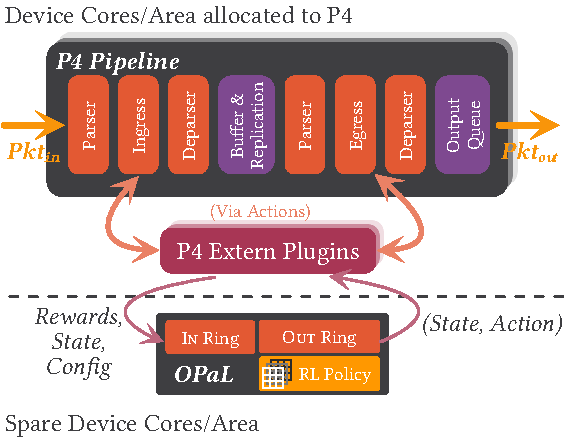
\includegraphics[keepaspectratio, width=0.85\linewidth]{diagrams/opal/arch-with-p4}
	\caption[\approachshort{}'s off-path interaction model with respect to a co-hosted P4 dataplane.]{SmartNIC-type \gls{acr:pdp} devices typically implement a target dataplane design by mapping the processing pipeline across one or more cores or \glspl{acr:fu}. Such devices are well-suited to this; \glspl{acr:npu} or \glspl{acr:soc} such as \glspl{acr:nfp} often have spare cores which aren't dedicated to running the dataplane, while spare area on \glspl{acr:fpga} may be used to design arbitrary \glspl{acr:fu}. While additional compute resources can relax the timing constraints needed to hit line-rate throughput, to prevent packet stalls as required we must move long-running computations (i.e., \gls{acr:rl} inference and updates) to this auxiliary compute. P4 programs expose device-specific functionality through \texttt{extern}s, allowing any extra compute resources and \gls{acr:ipc} to be accessed from ingress and egress tables, thus providing asynchronous execution and fast transmission of P4-extracted state as needed.\label{fig:netro-arch}}
%	\approachshort{} brings low-latency, online reinforcement learning directly to the dataplane. SoC- and NetFPGA-based SmartNIC devices expose spare compute---making in-situ, asynchronous processing and learning possible alongside P4 dataplanes. Classical RL policy methods are the key to making this computationally feasible. ?? REDO
\end{figure}

%?? 
%
%?? need to scale w/ available compute resources.
%
%?? need to not stall.
%
%?? Old, salesman-y.

\approachshort{} is a general, task-independent framework for in-network, online training and execution of \emph{any reinforcement learning agent design} using classical methods.
\approachshort{} is agnostic to the meaning of state vectors it receives as inputs and the actions it produces, which are employed by other functional units or the dataplane.
However, in-NIC/in-network execution specifically benefits packet-, flow-, and network-level learning, control, and optimisation tasks.
\approachshort{} meets the above goals by operating as a system which exists \emph{in parallel} to a co-hosted P4 dataplane.
\Cref{fig:netro-arch} describes and demonstrates the requisite interaction model; state extraction (i.e., flow telemetry collection and processing) occurs in the ingress and egress \glspl{acr:mat} of the P4 dataplane.
The packet pipeline of a P4 dataplane then communicates with \approachshort{} via \texttt{extern} plugins using \inring{} (state, configuration) messages to reconfigure the agent or request inference, and \outring{} (action) messages which carry output state-action pairs for the environment to make use of.
The contents of these messages are explained below.
To deploy this design, we require a platform-specific implementation of \approachshort{} itself and the \inring{}/\outring{} ring interaction mechanisms---exploiting how SmartNIC devices often expose general-purpose compute.
As many of these devices have engineering and development histories which predate P4, such general compute beyond the P4 \gls{acr:psa}'s limits~\parencite{p4-psa} is surprisingly common.
This then provides path-adjacent, on-chip \gls{acr:rl} in the dataplane.

\approachshort{} itself runs on one or more cores of a SmartNIC to convert state measurements of a known size from the environment into a stream of actions using a stored policy.
I discuss how it scales with additional compute as part of \cref{sec:opal-algorithm}.
%As an example, this might be to map flow state and performance measurements into a queueing priority for future packets from that flow, or to compute and apply a rate limit to preserve quality of service.
These dedicated cores are then responsible for processing requests, computing actions, and updating the underlying policy in real time.
Combined with reward measurements, this policy can then be updated or trained from scratch entirely on the \gls{acr:nic}, acting as a fully online \gls{acr:rl} agent.
An input state vector \emph{always} induces an action and, if online learning is desired, updates the policy using either an included reward or one retrieved from memory according to a key placed alongside the state.
This allows for simultaneous control and learning over independent systems by the same agent (i.e., optimising several flows with their own reward measures, such as \gls{acr:ddos} mitigation in an \gls{acr:as} where each next-hop \gls{acr:as} might have their own health metric).
Configuration messages may be provided over either the data or control-planes, where the P4 control plane may be used to provide access control over which machines or ports may send such commands.

%?? How does this meet the above requirements?
By executing on spare compute units, this design prevents packet stalling by moving longer-running compute out of the packet path, and can scale with cores made available at compile-time to improve latency and throughput.
By operating as closely as possible to the P4 pipeline, \approachshort{} uses and learns from per-packet state with minimal added latency (avoiding \gls{acr:pcie} transfers and batching as required), while imposing minimal impact on carried traffic for both bump-in-the-wire deployments and at end-points.
Moreover, the presence of the P4 dataplane allows easier inclusion of existing P4 traffic measurement and state extraction techniques, such as those covered in \cref{chap:nets}.


%unused device resources beyond the P4-PSA spec \emph{can and should be used} to drive asynchronous environmental control

%\Cref{fig:netro-arch,fig:single-and-parallel} outline our design and implementation on Netronome SmartNIC hardware in pursuit of this goal: unused device resources beyond the P4-PSA spec \emph{can and should be used} to drive asynchronous environmental control.
%We explain relevant NFP architectural details later in \cref{sec:netronome-platform-fundamentals}.
%\approachshort{} communicates with the packet pipeline of a P4 dataplane via \texttt{extern} plugins using \inring{} (state, configuration) and \outring{} (action) messages (\cref{fig:netro-arch}).
%Internally, \approachshort{} either has all its cores act independently (\cref{fig:single-and-parallel:single}) or cooperate to solve each task (\cref{fig:single-and-parallel:parallel})---with different latency-throughput benefits (\cref{sec:action-and-update-computation}).
%We open-source our firmware and control programs for the benefit of the community.
%Moving beyond the Netronome platform, we describe how our architecture may be adapted and improved on by bespoke hardware or FPGA-based deployment.

%However, high-speed data networks impose inviolable per-packet deadlines.

%To protect traffic throughput and allow effective deployment in as many environments as possible, \approachshort{} places RL execution on-chip, \emph{but off the main packet path}, communicating and running parallel to the main P4 dataplane.
%As shown in \cref{fig:netro-arch}, this asynchrony allows coexistence with P4 programs, and imposes minimal impact on carried traffic for both bump-in-the-wire deployments and at end-points.
%For instance, in the default deployment of a P4 packet processing pipeline on Netronome NFP chips several cores go unused (as does spare area on an FPGA design), making this paradigm possible.

\paragraph{Execution trace handling.}
To be generally applicable, we require that \approachshort{} is flexible in how reward values are mapped to input state vectors.
Target applications may aim to control one or many separate trajectories---i.e., learning from concurrent traces~\parencite{DBLP:conf/aamas/GroundsK07}---and in the online case we must have a low-overhead method of retrieving the correct last state-action-value tuple.
Moreover, each may require its own reward value depending on the nature of the \gls{acr:mdp}, for instance when optimising individual flow behaviour rather than joint control to benefit a shared environment.
\approachshort{} thus allows several sources for selecting these values, which may be configured separately for trace and reward selection:
\begin{description}
	\item[Shared.] A single \gls{acr:rl} trajectory or reward value is held. The reward value must be periodically updated using dedicated reward packets.
	\item[Field.] A given field of the input state vector is used as the lookup key (e.g., in a hash table) for either the trajectory or reward value. For instance, this may be a packet's flow hash or source \gls{acr:ip}. The reward value must be periodically updated as above.
	\item[Raw Field.] A given field of the input state vector is used as in \emph{Field}, but is not hashed for lookup.
	\item[Value.] A given field of the input state vector is directly used as the reward value. The installed policy can use or ignore this field as needed.
\end{description}

\paragraph{Policy constraints.}
To minimise (and predetermine) the amount of data required to encode a policy, as well as reduce the computational complexity of policy inference, tile coded policies are constrained in the following ways.
All tilings are assumed to be uniform rectilinear grids as in \cref{alg:tile-code}, where each dimension of input state has a single minimum and maximum assigned.
We assume that each dimension is subdivided into the same number of tiles, and that all tiling sets contain the same number of overlapping tilings over a given list of dimensions.
Each tiling set then covers a list of dimensions up to a platform-defined size.

\paragraph{Message formats.}
To provide the needed functionality and runtime configuration, \approachshort{}'s \inring{} ring receives the following message types.
\begin{description}
	\item[State messages.] These contain only a list of input data values from the environment, which invokes an inference and/or update cycle.
	\item[Reward messages.] These contain a single data value, and an optional data value used as a key to ensure it is mapped to the correct state trajectory.
	\item[Configuration.] These messages contain either top-level parameters (action counts, dimension counts, hyperparameters), or the dimension list for each tiling set.
	\item[Policy insertion.] As network packets have a restricted size, these messages subdivide a full policy parameter vector, and contain an array of tile value data alongside an \emph{offset} into the policy. These may be used to insert a pretrained policy into an offline agent, or to percolate policy updates among online learning agents in a network.
\end{description}
\approachshort{}'s \outring{} ring only carries a single message class, which is a state-action tuple.

%\begin{figure}
%	\centering
%\resizebox{0.48\linewidth}{!}{\begin{minted}{rust}
%type Tile = i32; /* or i16, or i8. */
%pub enum CtlMsg {
%    State(Vec<Tile>),
%    Reward(Tile),
%    Config(Config),
%    Insert{
%        offset: usize,
%        data: Vec<Tile>
%    },
%}
%
%pub enum Config {
%    Setup { .. },
%    Tiles { .. },
%}
%\end{minted}}
%\resizebox{0.48\linewidth}{!}{\begin{minted}{rust}
%type Tile = i32;
%pub enum CtlMsg {
%	State(Vec<Tile>),
%	Reward(Tile),
%	Config(Config),
%	Insert{
%		offset: usize,
%		data: Vec<Tile>
%	},
%}
%	
%pub enum Config {
%	Setup { .. },
%	Tiles { .. },
%}
%\end{minted}}
%	\caption[Sourec deo]{text}
%\end{figure}

\subsection{Data Format}\label{sec:opal-data-format}
%?? data format selection vs alternatives
To implement online learning such as in \gls{acr:rl}, we require a data type which allows us to perform numerical computation without an \gls{acr:fpu}---principally, to compute the values in action preference lists.
Moreover, to achieve online learning we require a format which is both fast to work with (to minimise processing latencies), and suited to represent gradients and temporal difference values i.e., incremental changes to stored policy weights.
Recalling the discussion in \cref{sec:numerical-representations-for-embedded-ml}, we employ \emph{fixed-point arithmetic}; it offers both the versatility needed to be easily reconfigurable, and it maps simply to \gls{acr:alu} operations.
For instance, only multiplications and additions require additional bitshifts for base pre-/post-conversion, while additions and subtractions require no additional overhead.\sidenote{Depending on the system design, (hyper-)parameters used only in divisions can be replaced with right bitshifts if we restrict their allowed values to negative powers of 2. This comes at the cost of system flexibility, and as such \approachshort{}'s implementation doesn't make use of this possibility.}

%?? Hence not binarised repr.
%?? Can choose bits allocated to fraction at runtime, overall bits at compile.
%?? Mention memory benefits.

From a configurability perspective, the count of fractional bits in a $Q$ number can be easily changed at runtime.
Naturally, this has no effect on overall latency and throughput of fixed-point arithmetic, but is a useful characteristic for being able to deploy different \gls{acr:rl} agents to the same hardware without invoking more costly firmware or \gls{acr:fpga} design installation.
If this is fixed at the same setting for all values used, then we needn't tag individual $Q$ numbers with information about their base, saving memory.
The bit width of the numbers themselves (i.e., $k$) may be changed only at compile time in many cases, particularly as SmartNICs often lack dynamic memory management in their native non-P4 programming environments.
Lower choices of $k$ sacrifice numeric range, but allow policies and data to occupy less memory---allowing fairer resource use versus other dataplane programs---and thus occupy less memory bandwidth in data transfers.
Alternatively, larger policies may be stored in the same memory bounds (potentially enabling the solution of more complex problems).

The reduced width and precision floating-point data formats we also examined earlier are not suitable here, in spite of their successes in other embedded domains.
First and foremost, these still require specialised \gls{acr:fpu} implementations.
This is naturally at odds with the design and goals of \gls{acr:pdp} hardware, and beyond \gls{acr:fpga} designs such a data format would be infeasible.
Software floating-point emulation has historically required \qtyrange{10}{30}{\times} more cycles to perform compared to hardware \glspl{acr:fpu}~\parencite{DBLP:conf/arith/IordacheT03}, which is incompatible with our need for low-latency and high-throughput processing.
While the added dynamic range would be useful in this application, performance is a primary goal.

\gls{acr:pdp} hardware excels in applying actions to network packets using \glspl{acr:mat}, potentially giving us a high-performance method to install selected actions within the network.
However, directly modifying these match tables from within the device itself is neither feasible nor safe.
On Netronome \gls{acr:nfp} hardware in particular, rule updates \emph{must} be applied by the co-hosted controller machine, as tables are reliant on the optimised DCFL~\parencite{DBLP:conf/infocom/TaylorT05} data format.
In addition to the prohibitive complexity of building this data structure on-device, its construction requires knowledge of the entire rule set (and cannot be incrementally updated).
I instead suggest in general that \texttt{extern}s or datapath stages which apply \gls{acr:rl} actions to packets should maintain a small store of state-action pairs, and periodically send these back to the controller for batch installation.
This ensures that the majority of installed rules benefit from faster hardware-accelerated lookups, while preventing installation delay on the newest decisions.
Platforms such as Intel Tofino greatly simplify this, where Tofino Native Architecture intrinsics such as \emph{Action Profiles/Selects} allow a P4 action to be chosen based on a register value (e.g., an \gls{acr:rl} action).

\subsection{Algorithm}\label{sec:opal-algorithm}
To enable online in-\gls{acr:nic} learning in spite of the computational limits of \gls{acr:pdp} hardware, we must return to \emph{classical} \gls{acr:rl} methods and models.
In particular, we focus on tile coding with one-step temporal-difference learning algorithms such as Sarsa, which were discussed and explained earlier (\cref{sec:tile-code} and \cref{sec:demo-rl-sarsa}).
%These choices have important benefits for in-NIC execution.
These functions do not require batches of inputs to learn in a stable way, negating the memory needed to store experience replays, and have simple update and inference logic.
Moreover, gradient computation is identical to the forward pass and has no dependency on the current parameter values $\wvec{}$, potentially allowing hit tiles to be stored to accelerate the next update step.
Finally, the choice of single-step algorithms (as opposed to $n$-step or Monte Carlo methods) bounds the amount of per-trace state required for online learning to just the last state-action pair, safeguarding the limited memory of our target devices.

As for how to take advantage of the multicore nature of SmartNICs, there are two strategies worth considering.
Suppose we have $n$ cores.
The first strategy is that we simply have each core work independently.
For instance, when dealing with a stream of input state vectors according to \approachshort{}'s interaction model, we may serve each arrived vector to a free core---this core then tile codes the state against every tiling, produces an output action, and then updates the policy as required (\cref{alg:tile-code,eqn:sg-sarsa}).
Intuitively, this produces an $n$~\unit{\times} throughput improvement assuming there are no bottlenecks at either the input and output queues or mutual exclusion around shared data.
However, this offers no reduction to the processing time of any \emph{individual} element---and so the state-action latency is not reduced as desired.

\begin{figure}
	\centering
	\resizebox{0.67\linewidth}{!}{
		\begin{tikzpicture}
	\node at (0,0) {
		\begin{tikzpicture}
			\draw[step=0.5cm,color=uofgcobalt,opacity=0.7,shift={(0,0)},label=above:{Tiling 0}] (-0.5,-0.5) grid (1,1);
			\fill[uofgcobalt,opacity=0.5] (0.5,-0.5) rectangle (1,0);
			\node[color=uofgcobalt] (t1g) at (0,1.2) {\footnotesize Tiling 1};
			
			\draw[step=0.5cm,color=uofgpumpkin,opacity=0.9,shift={(0.25,-0.25)},label=above:{Tiling 1}] (-0.5,-0.5) grid (1,1);
			\fill[uofgpumpkin,opacity=0.5,shift={(0.25,-0.25)}] (0,0) rectangle (0.5,0.5);
			\node[color=uofgpumpkin!50!uofgrust] (t2g) at (0.25,-0.95) {\footnotesize Tiling 2};
			
			\node[circle, black, draw,
			fill, radius=0.5pt, inner sep=0pt,minimum size=1.5pt, label=above:{$s$}] at (0.625,-0.125) {};
			%			\filldraw (0.625,-0.125) circle[radius=1.5pt,label=above:{$s$}];
			
			\draw[->] (-0.25,-0.5)--(-0.25,0.85);
			\draw[->] (-0.25,-0.5)--(1.1,-0.5);
			
			\node at (1,-0.7) {\footnotesize 1};
			\node at (-0.4,0.75) {\footnotesize 1};
			\node at (-0.35,-0.6) {\footnotesize 0};
		\end{tikzpicture}
	};
	
	\node (policy-head) at (2.5,1.2) {Policy};
	\draw[color=uofgcobalt,opacity=0.7] (2,0) rectangle ++(2,1) node[pos=.5] (t1p) {Tiling 1};
	\fill[uofgcobalt,opacity=0.25] (3.33,0) rectangle ++(0.67,0.33);
	
	\draw[color=uofgpumpkin,opacity=0.9] (2,-1) rectangle ++(2,1) node[pos=.5] (t2p) {Tiling 2};
	\fill[uofgpumpkin,opacity=0.25] (2.67,-0.67) rectangle ++(0.67,0.33);
	
	\draw (2,-2) rectangle ++(2,1) node[pos=.5] (tdot) {$\cdots$};
	
	\draw [->,color=uofgcobalt, bend left] (t1g) to (t1p.west);
	\draw [->,color=uofgpumpkin, bend right] (t2g) to (t2p.west);
	
	\node (act-list) at (1,-2.5) {$\mathbf{a}=\left[ \cdots \right]$};
	
	\draw [->, bend right] (t1p.west) to (act-list);
	\draw [->, bend right] (t2p.west) to (act-list);
	\draw [->, bend right] (tdot.west) to (act-list);
\end{tikzpicture}
	}
	\caption[A visualisation of how tile-coding can be split into subtasks as a map-reduce problem.]{Tile-coded function approximation can be considered as a map-reduce problem during both the inference and update steps. Action preferences are aggregated from \emph{disjoint} tile queries, where each tile hit contains a list of action values to add to $\mathbf{a}$. Retrieving or updating each tiling is thus a separate task. As all constituent action preference lists are disjoint between tasks, updating hit tiles requires no control over concurrent accesses---furthermore, it requires no final aggregation step.\label{fig:opal-par-tilecode}}
\end{figure}

To attain the latency improvements we desire, we must consider instead a second strategy: how several cores may work together to complete an individual inference or update operation.
Consider that tile coding computes individual hits against a set of tilings to produce a sparse boolean feature vector, which we'll denote $\mathbf{x}$, and refer to the set of all its non-zero indices by $H$.
Without loss of generality, suppose we have two tilings $t_1$ and $t_2$, with a number of tiles $|t_1|$ and $|t_2|$ in each respectively (such that $\dim{\mathbf{x}}=|t_1|+|t_2|$).
For notational simplicity, let each entry of an agent's policy data $\wvec{}$ be a vector of length $A$ (i.e., choosing between $A$ discrete actions).
A state vector will produce exactly one hit in each tiling, having indices $h_1\in[0,|t_1|)$ and $h_2\in[|t_1|,|t_1|+|t_2|)$, without overlap.
The final action preference list is given by \cref{eqn:lin-approx}, which we can specialise further:
$$
\mathbf{a} = \wvec{}^{\top} \mathbf{x} = \wvec{}\left[h_1\right] + \wvec{}\left[h_2\right] = \sum_{h\in{}H}\wvec{}\left[h\right]
$$
As a result, tile coded \gls{acr:rl} inference may be subdivided into several distinct computations tile indices whose results are added together as a final aggregation step.
Most of the work in each task arises from computing the tile index hit by the state vector.
Crucially, we have shown that memory regions of each tiling have no overlap with one another by construction.
Each memory address is visited and owned by exactly one task---hence, there is no concurrent access to policy values---and so no locks are required to protect each region of the policy.
\Cref{fig:opal-par-tilecode} demonstrates this process visually.

When updating the policy we need only monitor the number of completed tasks rather perform than a final aggregation step.
To see this, we specialise Sarsa's update step (\cref{eqn:sg-sarsa-update}) using our list of hit indices $H$.
After centrally computing a \gls{acr:td} value $\delta_t$ using $\mathbf{x}$ and a subsequent $\mathbf{x}'$, the action $a$ invoked by $\mathbf{x}$, and a learning rate $\alpha$, we update the policy values involved in the previous decision (using Python slice notation for simplicity):
\begin{align*}
\wvec{}\left[:,a\right] := \wvec{}\left[:,a\right] + \alpha\delta_t \mathbf{x}\\
\therefore~\wvec{}\left[h_1,a\right] := \wvec{}\left[h_1,a\right] + \alpha\delta_t,\\
\therefore~\wvec{}\left[h_2,a\right] := \wvec{}\left[h_2,a\right] + \alpha\delta_t.
\end{align*}
and so on for all $h \in H$ when we have an arbitrary number of tilings.
Thus, using the above knowledge that concurrent accesses to any parts of the policy cannot occur, an \gls{acr:rl} update divides into subtasks without locking in much the same fashion as inference does.

The aggregation step still risks becoming a bottleneck during inference; if individual preference lists are passed back as discrete messages, then this requires explicitly iterating over and summing all such lists.
While this may be performed by a dedicated worker thread or core in parallel to the other disaggregated inference tasks, this involves additional costs in every such task for \texttt{memcpy} operations into a message buffer.
Consider again that \approachshort{} targets \gls{acr:pdp} hardware: without a dynamic memory allocator, this buffer has bounded length and so risks causing head-of-line blocking for all other tasks.
However, encoding our values using a fixed-point representation allows us to employ atomic instructions to remove the aggregate step, thus producing a wait-free algorithm.
Recall that the aggregation step involves \emph{only additions}, that atomic integer fetch-add instructions are commonly offered on many machine architectures,\sidenote{While other datatypes such as \mintinline{rust}{f32} can technically support atomic operations on many platforms, outside of specialised \gls{acr:gpu} environments such as CUDA these incur non-trivial performance costs due to cache and register placement restrictions.} and that fixed-point addition is identical to integer addition.
As a result, the final action preference list may be allocated once and atomically added to by all workers.
Moreover, if extra care is required to prevent numeric overflows or ensure saturation, then any worker may locally verify whether the fetched value and summand would cause an overflow.
Alternately, an implementer may simply enforce upper and lower bounds on each action value to prevent positive or negative overflow.

\begin{algorithm}
	\caption{ParSa---\emph{Par}allel \emph{Sa}rsa\label{alg:parsa}}
	\SetKw{Let}{let}
	\SetKw{Enum}{enum}
	\SetKw{In}{in}
	\SetKw{Await}{await}
	\SetKw{Const}{const}
	\SetKwProg{parsa}{Function \emph{ParSa}}{}{end}
	\SetKwProg{control}{Function \emph{Ctl}}{}{end}
	\SetKwProg{minion}{Function \emph{Minion}}{}{end}
	\SetKwProg{tilecode}{Function \emph{TileCode}}{}{end}
	
	\tcc{Given message passing mechanisms \emph{scatter} and \emph{recv}, an input request stream \inring{}, an output action stream \outring{}, quantised arithmetic functions $Q_\mathit{mul}$ and TileCode, and omitting schedule/config/precache/reward updates.}
	\tcc{\emph{cfg}.$\alpha$, \emph{cfg}.$\gamma$ are hyperparameters affecting the significance of each update and the degree of forward-planning, respectively.}
	
	\Enum Par \{ Act(\emph{state}), Upd(\emph{delta, action, state}) \}\;
	\Const \emph{cfg, policy} = /* ... */\;
	
	\Let \emph{values}: [AtomicI32; \emph{cfg.n\_actions}] = \{0\}\;
	\Let \emph{acks}: AtomicI32 = 0\;
	\parsa{id, schedule}{\label{alg:parsa:par}
		\uIf{id==0}{\label{alg:parsa:parctl-start}
			\ForAll{state\_pkt \In \inring{}}{
				Ctl(\emph{state\_pkt})\;
			}
		}\label{alg:parsa:parctl-end}
		\Else{\label{alg:parsa:parminion-start}
			\While{true}{Minion(\emph{schedule}[$\mathit{id}- 1$], recv())\;}
		}\label{alg:parsa:parminion-end}
	}

	\control{state}{\label{alg:parsa:parctl-begin}
		\emph{values, acks} = \{0\}, scatter(Par::Act(\emph{state}))\;\label{alg:parsa:parctl-act}
		acquire slot for \outring, copy \emph{state} into slot\;\label{alg:parsa:parctl-preprep}
		\Await acks == \emph{cfg.n\_minions}\;\label{alg:parsa:parctl-await1}
		\Let \emph{action} = argmax(\emph{values})\;\label{alg:parsa:parctl-acchoose}
		write \emph{action} into \outring{} slot, enqueue\;\label{alg:parsa:parctl-acemit}
		\If{cfg.online}{
			\Let \emph{((l\_state, l\_act, l\_val), found\_s)} = \emph{cfg}.lookup\_state\_from\_key(\emph{state})\;\label{alg:parsa:parctl-checkstate}
			\Let \emph{(reward, found\_r)} = \emph{cfg}.lookup\_reward\_from\_key(\emph{state})\;\label{alg:parsa:parctl-checkreward}
			\If{found\_s \&\& found\_r}{
				\Let $\delta_t$ = $\mathit{reward} + Q_\mathit{mul}$(\emph{cfg}.$\gamma$, \emph{values}[\emph{action}]) $-$ \emph{l\_val}\;\label{alg:parsa:parctl-td1}
				$\delta_t$ = $Q_\mathit{mul}$(\emph{cfg}.$\alpha$, $\delta_t$)\;\label{alg:parsa:parctl-td2}
				\emph{acks} = 0, scatter(Par::Upd($\delta_t$, \emph{l\_act}, \emph{l\_state}))\;\label{alg:parsa:parctl-update}
				\Await acks == \emph{cfg.n\_minions}\;\label{alg:parsa:parctl-await2}
			}
			\emph{cfg}.store\_state(\emph{state}, \emph{action}, \emph{values}[\emph{action}])\;\label{alg:parsa:parctl-store}
		}
	}

	\minion{tasks, msg}{
		\Switch{msg}{
		\uCase{Par::Act(\emph{s})}{
			\ForAll{task \In tasks}{
				\Let \emph{hit} = TileCode(\emph{s}, \emph{task})\;\label{alg:parsa:parminion-acthit}
				\For{i \In [0..cfg.n\_actions)}{\label{alg:parsa:parminion-liststart}
					\emph{values}[\emph{i}].atomic\_add(\emph{policy}[\emph{hit}][\emph{i}])\;
				}\label{alg:parsa:parminion-listend}
			}
		}
		\uCase{Par::Upd($\delta$, \emph{a}, \emph{s})}{
			\ForAll{task \In tasks}{
				\Let \emph{hit} = TileCode(\emph{s}, \emph{task})\;\label{alg:parsa:parminion-acthit2}
				\emph{policy}[\emph{hit}][\emph{a}] += $\delta$\; \label{alg:parsa:parminion-update}
			}
		}
		}
		\emph{acks}.atomic\_add(1)\;\label{alg:parsa:parminion-lastack}
	}

%	\tilecode{state, task}{
%		\Let \emph{hit} = \emph{cfg}.get\_task(task)\;
%	}
\end{algorithm}

Parallelising the \gls{acr:rl} algorithm among processes in this way thus requires tight coupling between the function approximation and \gls{acr:rl} update algorithm.
The combination of all of these elements forms the basis of \emph{ParSa}---parallel Sarsa (\cref{alg:parsa}).
To match the deployment environment of SmartNIC devices, ParSa is presented such that each worker thread operates in an infinite loop to await and process requests delivered over a message channel \inring{}, and produce a stream of outputs on \outring{}.
We first assume that every process knows its own index---\emph{id}---and that a \emph{schedule} has been precomputed to divide individual tilings among cores as tasks (\cref{alg:parsa:par}).
This careful division is important; an individual tiling may contain several dimensions, and by recalling \cref{alg:tile-code} it is obvious that tilings with a higher dimension count require more iterations and are thus more expensive to infer.
To give some context on the number of tasks ParSa is expected to perform, a policy sized to match the agent designs from \cref{chap:ddos-rl} with one bias tile and \num{16} sets of \num{8} tilings creates \num{129} work items.
As such, a schedule is required to produce the most balanced workload between worker threads.\sidenote{Work stealing or other parallelisation strategies are not suitable choices for work balancing in tile coded Sarsa for several reasons. These include the computational simplicity of individual tasks, the predictable compute cost of any such task, and the relative cost of \gls{acr:ipc} required to pass cached state between workers.}
However, this is a deployment-specific implementation detail, as in addition to raw task costs an effective scheduler must account for cache size limits and physical/logical core differences.
I present an allocator tailored to Netronome hardware later in \cref{alg:parsa-schedule}.
A single worker thread, designated as the \emph{controller}, then receives and processes state vectors from the environment (\crefrange{alg:parsa:parctl-start}{alg:parsa:parctl-end}), while the remaining threads---\emph{minions}---retrieve a broadcast message of type \emph{Par} to apply over their prescheduled task set (\crefrange{alg:parsa:parminion-start}{alg:parsa:parminion-end}).

The \emph{Ctl} procedure directs tasks to minion threads, manages storage of execution traces, and computes the policy adjustments prescribed by the Sarsa \gls{acr:td} value.
Applying the insights of \textcite{DBLP:journals/firai/TravnikMSP18} to minimise action latency, an action is computed and sent out into the environment---and only then is the underlying policy updated.
For each input state, the controller thread zeroes out the shared aggregation space, where \emph{values} holds the aggregated action preference list and \emph{acks} contains the count of terminated minion threads.
An \emph{Act} request is then sent as a broadcast message to all minion threads using the platform-specific \emph{scatter} \gls{acr:ipc} call (\cref{alg:parsa:parctl-act}).
While the minions produce the action preference list asynchronously, the control thread then requests an output message slot and prepares it by copying the state into the acquired buffer (\cref{alg:parsa:parctl-preprep}).\sidenote{In principle, the controller thread may also act as another minion after this step, between scatter and recv calls, subject to code store limits.}
Once every thread has marked its termination, the values of each action given the input state are located in \emph{values} (\cref{alg:parsa:parctl-await1}).
The index of the largest value is then taken to be the chosen action, though this may be trivially modified to account for $\epsilon$-greedy selection (\cref{alg:parsa:parctl-acchoose}), which is then placed into the output message and returned to the environment (\cref{alg:parsa:parctl-acemit}).
When online learning is enabled, the control thread checks for a reward signal and prior state-action-value tuple according to the configured trace selection scheme from \cref{sec:opal-sys-model} (\crefrange{alg:parsa:parctl-checkstate}{alg:parsa:parctl-checkreward}).
If a match is found, it computes and reduces by $\alpha$ the Sarsa \gls{acr:td} value $\delta_t$ (\crefrange{alg:parsa:parctl-td1}{alg:parsa:parctl-td2}), before passing this adjustment and the prior state action pair to the minion threads to perform the update step (\crefrange{alg:parsa:parctl-update}{alg:parsa:parctl-await2}).
Modification to other single-step algorithms such as \emph{Q-learning} would be simple, requiring only changes to the computation of $\delta_t$.
The newest state-action-value tuple is then stored (\cref{alg:parsa:parctl-store}).

The \emph{Minion} procedure processes a single request to retrieve and aggregate, or update, the action values learned for an input state over some subset of the policy tilings, \emph{tasks}.
All minion threads cover the complete set of tilings between themselves.
In the case that action inference is requested, the policy hit index is computed against the input state for each tiling in this thread's task list (\cref{alg:parsa:parminion-acthit}).
As described above, each action value is atomically added to its matching position in the shared preference list \emph{values} (\crefrange{alg:parsa:parminion-liststart}{alg:parsa:parminion-listend}).
When an update is requested, all tile hit indices are recomputed (\cref{alg:parsa:parminion-acthit2}), and an adjustment $\delta$ is added to the selected action in each case (\cref{alg:parsa:parminion-update}).
Once all subtasks have been completed, this thread's completion is recorded (\cref{alg:parsa:parminion-lastack}).
While it is apparent that the indices of hit tiles may also be locklessly sent back and stored as part of the execution trace---i.e., by adding an extra value slot per task---the number of subtasks often far exceeds the count values in a state vector.
As a result, this results in a larger \texttt{memcpy} in \emph{Ctl} (the serial portion of ParSa), and as such it is more efficient to recompute hit indices in the update step---though this optimisation is useful in the case of the first (non-ParSa) parallelisation strategy.

%?? mention that theoretical worse than just adding more cores due to message passing costs, memfence, compiler reordering etc., size of serial portion, number of constituent tasks. (could split to indiv actions, but need stupid cores for feasible.)
As required, this new algorithm scales with increasing processor counts to reduce both the inference and update costs incurred by a single state vector.
This lowers the state-action latency and produces a corresponding increase to throughput.
However, the factor of speedup is \emph{worse} than $n$~\unit{\times}, and exhibits diminishing returns in terms of core count---for instance due to the cost of \texttt{memcpy}s and arithmetic in the serial logic of \emph{Ctl}, message passing costs at the broadcast and receive steps, and any memory fences or reorderings inserted by the compiler around atomic arithmetic.
This is limited further by the number of subtasks which can be generated for a given policy.
While ParSa assumes tile-level granularity, it may be modified to compute individual actions at the cost of being dominated by significant repetition of work and \gls{acr:ipc} overheads.
Since these aspects are platform-dependent, this behaviour can only be shown empirically as in \cref{sec:opal-results-work-alloc}.

\section{Implementation}\label{sec:opal-impl}
We implement \approachshort{} on... ?? Netronome...
?? What else do we cover.

?? As the allocation of cores/chip area is set ahead of time by a framework or system administrator, \approachshort{}(-\Coopfw) agents enumerate themselves at runtime, during initialisation.

?? We open-source our firmware and control programs for the benefit of the community.
Moving beyond the Netronome platform, we describe how our architecture may be adapted and improved on by bespoke hardware or FPGA-based deployment.

?? \approachshort{} communicates with the packet pipeline of a P4 dataplane via \texttt{extern} plugins using \inring{} (state, configuration) and \outring{} (action) messages (\cref{fig:netro-arch}).
Internally, \approachshort{} either has all its cores act independently (\cref{fig:single-and-parallel:single}) or cooperate to solve each task (\cref{fig:single-and-parallel:parallel})---with different latency-throughput benefits (\cref{sec:action-and-update-computation}).

\subsection{Action and Update Computation}\label{sec:action-and-update-computation}
\approachshort{} applies the insights of \textcite{DBLP:journals/firai/TravnikMSP18} to minimise action latency; an action is computed, sent out into the environment, and only then is the underlying policy updated.
Using one of the below strategies chosen at compile time, a state vector is tile coded, converted into action probabilities, and an action is chosen.
This is then written out to the environment as in \cref{sec:agent-environment-communication}.
If online learning is enabled, \approachshort{} then checks an internal hashmap for a previous state-action pair matching the current instruction source, and if found then the policy is updated.
Updates are computed using \emph{single-step semi-gradient Sarsa}~\cite[pp. \numrange{217}{221}]{RL2E}, though modification to support other single-step methods would be trivial.
The new state- or tiles-action pair is then written into storage.
\approachshort{} can be configured to automatically select values of the input state vector as keys for state and reward storage.

Two firmware models govern how the compute-heavy parts of these tasks (action selection, policy updates) are carried out:
\begin{description}
	\item[\Indfw{} (\cref{fig:single-and-parallel:single})] Separate threads listen for new states, and each performs its work sequentially. Computing an action list requires a \emph{read lock} on the policy. If an update occurs, the core requests a \emph{write lock} before updating, greatly limiting online throughput. \emph{Tile lists} are stored for update computation.
	\item[\Coopfw{} (\cref{fig:single-and-parallel:parallel,alg:parsa})] Threads cooperate on processing state vectors, minimising latency. \emph{Minion} threads have a fixed list of work items, while a \emph{controller} thread sends compute/update commands before awaiting worker completion. Work items are disjoint, requiring no policy locks. \emph{State vectors} are stored for update computation.
\end{description}
Each offers a different point of optimisation; if updates are disabled, then the \indfw{} model can maximise throughput, while the \coopfw{} model is designed to minimise decision latency and needs no locks to update the policy (increasing \emph{online learning} throughput).
These correspond to only executing a trained policy and actively (re-)training a policy, respectively.
%ParSa is described here at a high level, as an algorithm suited for \emph{any multiprocessor environment}.
%We omit the simple logic for $\epsilon$-greedy action selection (which we implement), and note that modification to other single-step algorithms such as \emph{Q-learning} would be trivial.
%We detail our communication primitives in \cref{sec:intra-agent-communication}, and our work scheduling strategy in \cref{sec:work-allocation}, eliding the details of tile-coding as they are well-understood.
%In general it is also possible for the \emph{Ctl} task to act as an additional \emph{Minion} in its parallel sections; we were limited here by code store requirements on the NFP.
Latency and throughput, as in many networked systems, have different effects upon RL agents according to their design and target problem.
Higher RL throughput is a necessity for per-flow or per-packet applications, which can require high decision-per-second rates even after combining state measurements received from the environment, such as flow control in DDoS prevention.
Equally, lower latency affords an agent finer-grained control and learning of a problem, being able to react sooner to new information (e.g., device state in a routing optimisation problem, or queue depth when trying to enforce packet pacing).

Paradoxically, we found that in the general \emph{ParSa} algorithm it was more efficient \emph{to do more work} by having each worker recompute its tile subset from a stored state.
It transpired that cacheing this data placed a larger \texttt{memcpy} in the serial section, whose size did not scale at all with bit depth.
Additionally, we do not use bitshifts in place of division operations in our implementation, due to the strict limits that power-of-two tile widths place upon policy design.

\subsection{Agent-Environment Communication}\label{sec:agent-environment-communication}
\approachshort{} uses \emph{multiple-producer/multiple-consumer} (MPMC) messaging channels to communicate with other elements; be they P4 programs on the packet path, or other on-chip analysis and control modules.
Through these channels a system \emph{pushes} state vectors, reward measures, and setup packets as inputs, and \emph{pulls} a stream of state-action pairs as outputs.
This allows decisions to be made asynchronously---preventing packet stalling---and allowing many RL agents to be used if desired.
The key insight of this mechanism is that on-chip reward/state signals enjoy first-class support in the same manner as packets from the P4 dataplane, allowing agents to act on environmental signals from other on-NIC/chip asynchronous processes or the controller.
As such, \approachshort{} can receive input from P4 \texttt{extern}s or other, dedicated off-path flow state measurement applications.

Our implementation uses platform-specific IPC (\emph{EMEM ring buffers}) with hardware signalling on work arrival to achieve this.
As PDP hardware lacks dynamic memory allocation, P4 pipeline threads request buffers for packet payloads using a shared freelist to enable state/configuration/policy data handover.
Packet headers are extracted and parsed using the tooling autogenerated by the P4 pipeline.
We found that this costs a median \qtyrange{126}{140}{\nano\second} communication time (local--remote), comparable to message channels in the Rust and Go languages on commodity hardware.

%The main interaction model is that platform-specific IPC (message rings) is used to \emph{push} configuration, state vectors, and reward measurements to the RL system.
%These same mechanisms are used by other cores on the same device to \emph{pull} output actions from the RL system.
%Both input and output can occur on any other core of the device, i.e., as part of P4 \texttt{extern} plugins or a dedicated flow state measurement subsystem, while the P4 control plane itself provides granular control over which flows are monitored or affected.

\subsection{Intra-Agent Communication}\label{sec:intra-agent-communication}
Even with parallel problems such as \emph{ParSa}, optimising for latency requires meticulous care in how work is passed out and aggregated.
This is truer still when moving from the moderately fine-grained control of classical RL ($\sim$\qty{1}{\milli\second}) to its logical limit (tens of \si{\micro\second}).
Ordinarily, the marshalling of requests, responses, and shared data access can incur significant overheads.
On-chip execution and the nature of action preference computation allow us to use lockless atomic aggregation, removing the overheads of explicit messaging/packetisation.
Moreover, adjacent functional units/cores often have special-purpose shared registers or share a small fast cache to accelerate communication.

?? \cref{fig:single-and-parallel}
Internally, \approachshort{} either has all its cores act independently (\cref{fig:single-and-parallel:single}) or cooperate to solve each task (\cref{fig:single-and-parallel:parallel})---with different latency-throughput benefits (\cref{sec:action-and-update-computation}).

\begin{figure}
	\centering
	\begin{subfigure}{\linewidth}
		\centering
		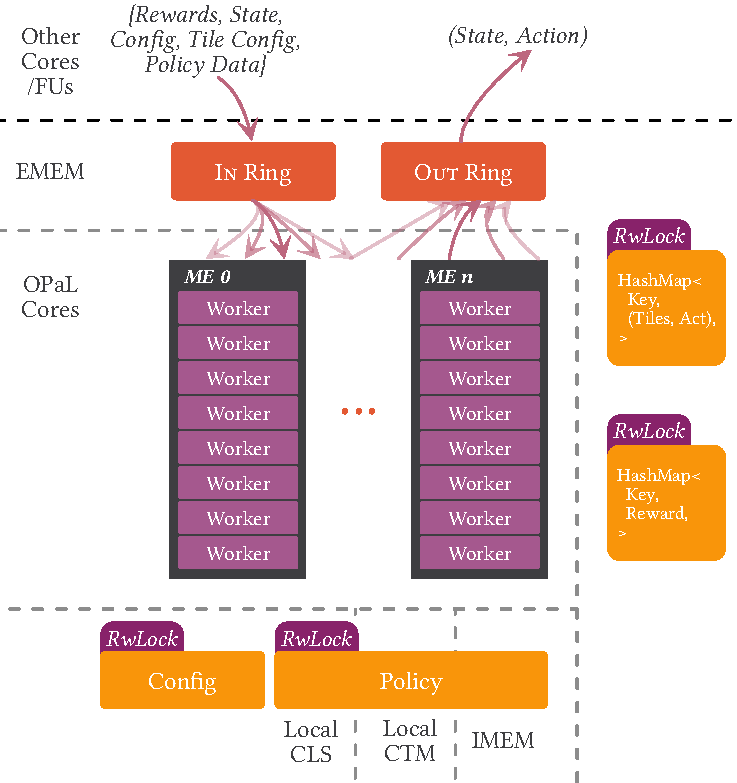
\includegraphics[keepaspectratio, width=0.78\linewidth]{diagrams/opal/ind}
		\caption{\Indfw{} (offline throughput-optimal). \emph{Workers} independently pull commands from (and push actions to) the environment, locking policy access for updates.\label{fig:single-and-parallel:single}}
	\end{subfigure}

	\begin{subfigure}{\linewidth}
		\centering
		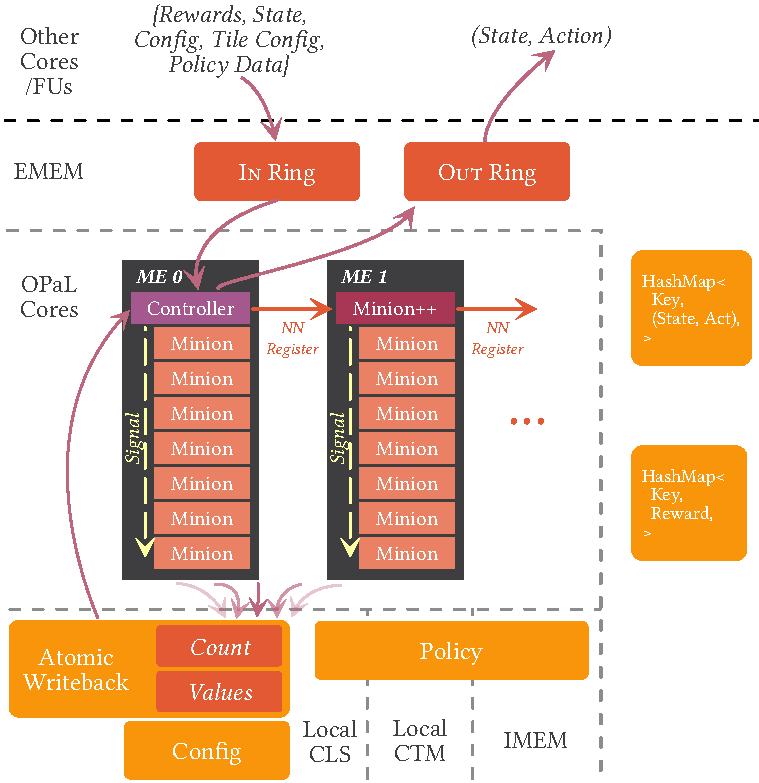
\includegraphics[keepaspectratio, width=0.8\linewidth]{diagrams/opal/coop}
		\caption{\Coopfw{} (online-optimal). A single \emph{controller} delegates RL computation and updates to many \emph{minion} threads, who operate on independent subtasks.\label{fig:single-and-parallel:parallel}}
	\end{subfigure}
	\caption{\approachshort{}'s compute strategies scale to fit device capacity according to either latency or throughput needs.\label{fig:single-and-parallel}}
\end{figure}

%?? reduce below and make take-homes more generic if possible

Our implementation exploits the locality of cores in the NFP, which can be factored into designs on other platforms like NetFPGA.
Policy compute/update/configure tasks are passed between cores using direct \emph{next neighbour} registers, signalling all child threads in response.
Such on-chip signals cost just $\sim$\qty{20}{\nano\second} per relayed message.
Each core performs atomic adds to a shared preference list and an acknowledgement counter checked by the master thread, implementing our wait-free \emph{ParSa} algorithm (\cref{alg:parsa}).
This is essential for aggregation compared to the use of bounded message buffers, which caused significant head-of-line blocking.

%On-chip local messages cost us just $\sim$\qty{20}{\nano\second} latency per relayed message
%
%In earlier designs we had experimented with bounded buffers as in \cref{sec:agent-environment-communication} for this, modified to be located solely in CLS memory, dedicating the master thread to result aggregation.
%We found that this created a performance bottleneck at this final stage, causing significant head-of-line blocking for each of the workers.
%Similarly, our next neighbour work notification scheme ($\sim$\qty{20}{\nano\second} latency per relayed message) was examined against \emph{reflector} and \emph{work queue} IPC mechanisms (\qtylist{58;126}{\nano\second} per messaged core).
%These slower messages can be used in theory to skip ahead into longer ME chains.

%Our implementation exploits the locality of threads, cores, and their parent islands in the NFP architecture.
%Policy compute/update tasks and configuration updates are passed between cores using these direct \emph{next neighbour} registers, signalling all child threads in response.
%Each task performs atomic adds to a shared preference list, and atomically increments an acknowledgement counter to be periodically checked by the master thread, implementing the wait-free \emph{ParSa} algorithm we introduce (\cref{alg:parsa}).

%In earlier designs we had experimented with bounded buffers as in \cref{sec:agent-environment-communication} for this, modified to be located solely in CLS memory, dedicating the master thread to result aggregation.
%We found that this created a performance bottleneck at this final stage, causing significant head-of-line blocking for each of the workers.
%Similarly, our next neighbour work notification scheme ($\sim$\qty{20}{\nano\second} latency per relayed message) was examined against \emph{reflector} and \emph{work queue} IPC mechanisms (\qtylist{58;126}{\nano\second} per messaged core).
%These slower messages can be used in theory to skip ahead into longer ME chains.

\subsection{Reconfigurability}
\approachshort{} allows policy design and algorithmic learning parameters to be changed at runtime using at most two control packets.
For instance, design changes are useful at the end of learning (moving from online to offline), or when trying to train a new policy for another problem from the same vantage point.
Parameter changes are useful when an online agent must become more (or less) adaptive to new data (i.e., after detecting a changepoint in traffic).
This extends to policy data, which may be imported from a pre-trained model via such packets and exported via PCIe to the host machine.
Some aspects must be chosen at compile time; bit depth, \Coopfw/\Indfw, and maximum policy/tiling/state sizes---these govern core operation or allocated memory.
Choosing a bit depth of \qtylist[list-pair-separator = { or }]{16;8}{\bit} halves/quarters policy memory costs, allowing more complex problems to be modelled using more dimensions or fine-grained tiles.

In our implementation, configuration packets are carried over UDP and signalled to the P4 parser using a reserved (pool 2~\parencite{rfc2474}) DSCP value as used by \textcite{DBLP:conf/isca/LiLYCSH19}.
While this mainly automates parser generation, it also allows for configuration to be received from only trusted hosts (over the dataplane if needed) via P4 rules.
Our control packet generation library and evaluation frameworks which build upon it are written in Rust.

%Runtime reconfiguration and interaction occur via the control and/or dataplane: the ease of use of the P4 pipeline's match-action tables and custom protocol parsers, combined with the dedicated input pipe to the NIC's controller (the host machine), allow these to be cleanly separated or combined as needed.
%Bit depth of quantised measurements/preferences, maximum policy sizes, and parallelisation strategy may be configured at compile time.

\subsection{Work Allocation}\label{sec:work-allocation}
Due to the lack of dynamic memory allocation on PDP hardware, and to simplify value lookups, policies cannot be stored sparsely.
As a consequence, tiling space requirements scale exponentially with dimension count, and so higher-dimension tilings must be placed in larger (and slower) memory regions.
As a result, in many architectures policy parameters are split across such regions, giving different access and compute costs to different tasks.

We use a simple first-fit work placement algorithm run in \approachshort{}, placing the largest work item into the least loaded thread of the least loaded core (as the NFP uses hardware threads).
Each work item is a separate \emph{tiling} over a list of dimensions, noting that many such tilings may be grouped into a set (using different offsets for smoother coverage of the state space).
The cost of any work item (from its dimension count and memory location) was empirically measured offline, and we weigh the total cost per core based on the number of minion threads available.
This weighting specifically accounts for the controller thread on the first core.
Work allocation and cached per-item data are recomputed when policy configuration is installed or changed.
Naturally, for $n$ tilings and $m$ threads this procedure is $\mathcal{O}{\left(n\log{m}\right)}$: two find/update min operations into binary heaps per tiling, storing $m/8$ and $\le8$ costs respectively.

%\subsection{Variable Quantisation Bit Depth}
%At compile-time, \approachshort{} can be configured to use \qtylist[list-final-separator = { or }]{32;16;8}{\bit} values in input states and its internal policies.
%Naturally, smaller bit depths reduce the storage required for policies, tiling data, and stored state-action pairs---allowing more complex problems to be modelled using more dimensions or fine-grained policies.
%Through the lens of computational efficiency, reduced bit depth should allows action preference lists to be read using fewer I/O operations (as more values may fit into a single machine word).
%
%We had investigated bit-stuffing several such values into a single word for our atomic writeback mechanism (as the platform offers both \qtylist{32;64
%}{\bit} atomic addition).
%This is analogous to SIMD---through clever use of padding bits---but we found that manipulating tiles into the correct format added \qty{10}{\percent} extra overhead.
%We investigate further performance implications of changing bit depth in the sequel.

%Potential: low-latency train for some specific points, and high throughput for others? Think on the exact note I took...
%
%``can have accel'd offline, train online subset w/ my approach''
%
%THis might mean "do 32-bit online", then downsample to 8-bit policy for high-throughput mode.
%
%Can changes in trained policy be used to transfer to a more complex function approximator elsewhere?

\subsection{Limitations}\label{sec:limitations}
Unfortunately, direct rule installation into P4 tables from the SmartNIC itself is not, in general, possible.
To achieve line-rate match-action table lookup, platforms like NFP use accelerated datastructures (e.g., DCFL~\parencite{DBLP:conf/infocom/TaylorT05}) which must be computed by the controller over the \emph{entire rule set}.
Even through \texttt{extern}s, directly adding new rules is neither feasible nor safe.
We instead suggest on NFP chips that \texttt{extern}s or datapath stages which apply RL actions to packets should maintain a small store of state-action pairs, and periodically send these back to the controller for batch installation.
This ensures that the majority of installed rules exhibit accelerated performance, while preventing installation delay on the newest decisions.
Platforms such as Intel Tofino greatly simplify this, with Tofino Native Architecture intrinsics such as \emph{Action Profiles/Selects} allowing a P4 action to be chosen based on a register value (i.e., an RL action).

%As is expected of parallel algorithms, efficient division of work, communication, and aggregation add per-task overheads in both the serial and parallel portions.
Efficient division of work, communication, and aggregation add per-task overheads in both the serial and parallel portions.
Even in wait-free algorithms, this requires a minimum number of workers to improve upon the latency bounds of a serial approach.
We investigate the exact worker count requirements imposed to break even or improve upon single-threaded execution in \cref{sec:results}.

\subsection{Targeting other device classes}
While this design caters to Netronome devices, many aspects have clear analogues in other SmartNICs, such as the NetFPGA SUME.
For instance, additional off-path functional units can serve as workers, like the floating-point adders used by \textcite{DBLP:conf/isca/LiLYCSH19}.
Rather than general-purpose IPC, \approachshort{} would be hard-wired between internal workers and to the P4$\rightarrow$NetFPGA~\parencite{DBLP:conf/fpga/IbanezBMZ19} actions that interface with it.
%Further optimisations arise from this model: a NetFPGA design would be able to replicate and optimise further on this concept of dedicated, low-latency communication between functional units.
As we show later, using a bit depth below the native word size reduces overall efficiency.
%This reduces overall efficiency even though considerably fewer reads are made.
We expect an FPGA design would allow this to match the desired bit depth and enable the SIMD-like optimisations we discuss without creative and costly bit-stuffing.

Bringing \approachshort{} to PDP switches such as the Tofino is difficult as they closely match the P4-PSA, leaving no spare general-purpose compute units.
Taking inspiration from real-time programming, a potential solution is to divide RL processing across several packets (i.e., computing a portion of the preference list each time) until further work would delay outbound transmission.
This would introduce new issues in concurrent access, work splitting, and altered timescales for learning: we leave their treatment to future work.

%While specifics of this design cater to Netronome devices, many aspects have clear analogues in NICs of similar form-factor, such as the NetFPGA SUME platform.
%For instance, other cores can be introduced by designing additional off-path functional units,  like the floating-point adders used by \textcite{DBLP:conf/isca/LiLYCSH19}.
%Rather than general-purpose IPC, \approachshort{} would be hard-wired between internal workers and to the custom actions that interface with it, using the P4$\rightarrow$NetFPGA toolchain to offer granular control over packet and flow selection.
%%Further optimisations arise from this model: a NetFPGA design would be able to replicate and optimise further on this concept of dedicated, low-latency communication between functional units.
%As our later results show, using a bit depth below the native word size forces the compiler to emit excess code to extract and re-align preference values, reducing overall efficiency.
%%This reduces overall efficiency even though considerably fewer reads are made.
%We expect that a more bespoke hardware/FPGA design would allow this to match the desired bit depth and enable SIMD-like optimisations we discuss without creative and costly bit-stuffing.
%
%Bringing \approachshort{} to high-port density devices such as Tofino-powered switches is more difficult.
%As discussed in \cref{sec:motivation}, Tofino ASICs map closely to the P4 PSA, meaning that there are no spare asynchronous general-purpose compute units to place this work on.
%Taking inspiration from real-time programming techniques, a potential solution is to divide RL actions across several received packets (i.e., iteratively computing a portion of the action preference list each time) until any further work would delay outbound transmission.
%This, however, would introduce new issues surrounding concurrent accesses, work splitting, and altered timescales for learning: we leave their treatment and examination to future work.

\section{Evaluation}\label{sec:opal-evaluation}
%Traffic is played back from hosts via Tcpreplay at a bandwidth assigned uniformly from a `good' or `bad' distribution, each using the same pcap file with source and destination IP addresses rewritten.

This work is most naturally compared against Marl, introduced by \textcite{DBLP:journals/eaai/MalialisK15}, the state-of-the-art in \gls{acr:rl}-based \gls{acr:ddos} prevention.
We are most interested in seeing how their approach contrasts with the new agent designs across different topologies and workloads.
Different network environments will also impose different levels of host density, where popular web servers may have orders of magnitude more clients than egress points from their network---I aim to show how these characteristics affect performance and learning rate.
Marl is known to outperform the AIMD~\parencite{DBLP:journals/ton/YauLLY05} strategy, yet the state of the art has long since moved on.
To paint a more current picture, I compare this work against an effective modern approach, \emph{SPIFFY}~\parencite{DBLP:conf/ndss/KangGS16}.
SPIFFY tests a proportion of flows by routing them through an alternate path with higher bandwidth, observing how their speed changes some time later.
This comparison lets us position our new agent designs against the state of the art, observing that SPIFFY has a similar mode of interaction to \gls{acr:rl}-based systems (taking action, observing an effect, and acting once again) and does not rely on protocol characteristics or signatures.
In reimplementing SPIFFY, I make the simplifying assumption that a suitable unused path exists (with identical bandwidth to the server's link).
\qty{10}{\percent} of active flows were tested at a time (according to the authors' observation that there is a factor of \qty{10}{\times} difference between the ideal and achieved bandwidth expansion), excluding flows below \qty{50}{\kilo\bit\per\second} and requiring a \qty{3}{\times} expansion from legitimate flows, making a judgement after \qty{5}{\second}.

To test this, I made use of both traffic models introduced in \cref{sec:a-new-normal} (Opus and \gls{acr:tcp}), both topologies discussed below (1-dest vs.\ Fat-Tree), and vary the amount of hosts typically communicating over each agent's ingress/egress node.
Additionally, these new models were evaluated in multi-agent mode (\emph{separate}, no model sharing), and in single-agent mode (\emph{single}, zero-cost perfect information sharing).
In each case, the algorithm's performance was averaged over \num{10} episodes of length \num{10000} timesteps (setting each agent's $\wvec{}=\mathbf{0}$ between episodes).
Host allocations at the beginning of each episode were generated pseudorandomly to ensure fairness between episodes---a host is malicious with probability $\operatorname{P}\left(\mathit{malicious}\right)$, and is benign otherwise.
Benign hosts generate traffic according to either \cref{sec:tcp-http-traffic-model,sec:udp-opus-traffic-model} depending on the experiment, while malicious hosts generate traffic as described in \cref{sec:attack-traffic-model} (both at experiment-dependent rates).

All experiments were executed on Ubuntu 18.04.2 LTS (GNU/Linux 4.4.3-040403-generic x86\_64), using an Intel Core i7-6700K (\qtyproduct[product-units=single]{4 x 4.2}{\giga\hertz}) which had \SI{32}{\gibi\byte} of \gls{acr:ram}.
%All code underpinning these findings is available on a public repository\footnote{\url{https://github.com/FelixMcFelix/rln-dc-ddos-paper}}.
%All code underpinning these findings is available on a public repository.\footnote{Private until publication.}

\subsection{Single destination}\label{sec:single-dest}
%?? Move description of tree topol to here.
The network is tree-structured, where one server $s$ connects through a dedicated switch to $k$ team leader switches, each connected to $\ell$ intermediate switches, which in turn each connect to $m$ egress switches.
We then have $N_{\mathit{hosts}} = k \ell m n$.
\Cref{fig:marl-topol} demonstrates this.
%Although \citeauthor{DBLP:journals/ccr/MahajanBFIPS02a}, the originators of this topology, make it clear that it exists as a fairly unrepresentative example \cite{DBLP:journals/ccr/MahajanBFIPS02a}, it remains the case that such a network topology allows for functional testing, and indeed is illustrative of one way in which attack traffic might aggregate in the network.
%It is hard, however, to argue its relevance to specific classes of victim or to reason about the interactions it might have with dependent applications.
%We aim to address this through \cref{sec:performance-in-an-emulated-environment}.
The network topology was configured using $k=2$ teams, $\ell=3$ intermediate nodes per team, $m=2$ agents per intermediate node, and $n \in \{2, 4, 8, 16\}$ hosts per learner.
This is a slight simplification of \Textcite{DBLP:journals/eaai/MalialisK15}'s \textquote{online} experiment, choosing fewer teams but remaining as a single server with a fan-out network.
%The algorithm parameters were set at $\gamma=0$ (leading to opportunistic behaviour), $\alpha=0.05$, having linearly annealed $\epsilon=0.2 \rightarrow 0$ by $t=3000$.
%Benign and malicious hosts uploaded between \SIrange{0}{1}{\mega\bit\per\second} and \SIrange{2.5}{6}{\mega\bit\per\second} respectively, and hosts were redrawn at each episode's start with $\operatorname{P}(\mathit{malicious})=0.4$.
%$U_s$  $k \ell mn+2$ \si{\mega\bit\per\second}.
%The performance of each choice of $n$ was averaged over \num{10} episodes of length \num{10000} timesteps (setting each agent's $\wvec{}=\bm{0}$ between episodes).
%Host allocations were generated pseudorandomly to ensure fairness between choices of $n$.
%These parameter choices match those of the original study to enable direct comparison, and are (to the best of our knowledge) arbitrary, but we justify our range of $n$ as capturing increasing scales of host activity.

\begin{figure}
	\centering
	\resizebox{0.9\linewidth}{!}{\begin{tikzpicture}[
	texts/.style = {text=black},
	labeltexts/.style = {text=uofgsandstone},
	treeline/.style = {draw=uofgburgundy},
	treenode/.style = {texts, circle, centered, fill=white, treeline},
	load/.style = {fill=uofgcobalt},
	loadhide/.style = {fill=uofgcobalt!40!white},
	external/.style = {fill=uofgrust},
	externalhide/.style = {fill=uofgrust!40!white},
	hideline/.style = {draw=uofgsandstone!40!white},
	hidenode/.style = {treenode, hideline},
	grow'=right
]
	\node[treenode, label={[texts]above:Server}] (root) {}
	child [treeline] { node [treenode, label={[texts]above:Core}] (sswitch) {}
		child [treeline] { node [treenode, label={[texts]above:Leader}] (teaml) {} 
			child [treeline] { node [treenode, label={[texts]above:Intermediate}] (inter) {}
				child [treeline] { node [treenode, load, label={[texts]above:Agent/Egress}] (agent) {}
					child [treeline] { node [treenode, external] (extern) {}
						child [treeline] { node [treenode, external, label={[texts]above:Host}] (host) {} }
						child [hideline] { node [hidenode, externalhide] (endhost) {} }
					}
				}
				child [hideline] { node [hidenode, loadhide] (endagent) {} }
			}
			child [hideline] { node [hidenode] (endinter) {} }
		}
		child [hideline] { node [hidenode] (endteaml) {} }
		edge from parent
		node[below, labeltexts] {$U_s$}
	};
	
	%\draw[-] (teaml) -- (endteaml);
	\node [labeltexts] (kdots) at ($(teaml)!0.5!(endteaml)$) {$\rvdots$};
	\node [labeltexts, right = -0.1cm of kdots] {$k$};
	\node [labeltexts] (ldots) at ($(inter)!0.5!(endinter)$) {$\rvdots$};
	\node [labeltexts, right = -0.1cm of ldots] {$\ell$};
	\node [labeltexts] (mdots) at ($(agent)!0.5!(endagent)$) {$\rvdots$};
	\node [labeltexts, right = -0.1cm of mdots] {$m$};
	\node [labeltexts] (ndots) at ($(host)!0.5!(endhost)$) {$\rvdots$};
	\node [labeltexts, right = -0.1cm of ndots] {$n$};
\end{tikzpicture}}
	\caption[Tree-structured network topology diagram for evaluating a single-destination network.]{
		Network topology diagram, showing how the server and its core switch's $k$ teams are structured, with $\ell$ intermediate routers per team, connected to $m$ agents which each moderate $n$ hosts beyond a single external switch.
		%	Empty nodes are considered to be internal.
		Red nodes are external, and each blue node hosts an agent.
		\label{fig:marl-topol}
	}
\end{figure}

\subsection{Multiple destinations}
The previous topology allows for direct comparison against the state-of-the-art, and indeed is illustrative of one way in which attack traffic might aggregate in the network.
It is hard, however, to argue its relevance to specific classes of victim or to reason about the interactions it might have with dependent applications.
In contrast, the fat-tree topology~\parencite{DBLP:conf/sigcomm/Al-FaresLV08} sees regular use in real-world data centres and scales well horizontally.
%?? Come up with description of fat-tree (multi-dest) topol.
%?? Why fat tree? regularly appears in modern datacentres.
%?? $k=4$ fat-tree , with one pod hosting two servers $s_0,s_1$.
We use a $k=4$ fat-tree, with one pod hosting two servers $s_0$ and $s_1$.
$n$ external hosts connect through each core switch (where agents are hosted), and communicate with $s_0, s_1$ uniformly randomly.
Both servers host identical services.
We set $n \in \{6, 12, 24, 48\}$ hosts per learner (keeping $N_{\mathit{hosts}}$ identical to each tier of the single-host topology), and restrict $U_{s_0} = U_{s_1} = U_s / 2$.

\subsection{Parameters}
The algorithm parameters were set at $\alpha=$~\num{0.05}, linearly annealing $\epsilon=$ \num{0.2} $\rightarrow$ 0 by $t=$~\num{3000} in the case of Marl (\num{8000} actions per agent in the \emph{Instant/Guarded} models).

Benign hosts each occupied \qtyrange{0}{1}{\mega\bit\per\second}, and hosts were redrawn at each episode's start with $\operatorname{P}(\mathit{malicious})=$~\num{0.4}.
%The original introduction of this approach to direct-control reinforcement learning as introduced by \textcite{DBLP:journals/eaai/MalialisK15} fails to consider key cases: the absence of a suitable heuristic classifier $g(\cdot)$, disjoint ranges of traffic distribution (i.e., the presence of benign heavy-hitters), the accurate simulation of TCP-like behaviour (and its effects on collateral damage), and high densities of hosts at egress points.
%?? Why? ...
%Of these, the latter two are most deserving of a closer investigation, as they have stronger implications for wide-scale deployment.
%These are important issues, particularly when we consider real-world deployment.
%Heuristic estimates of traffic legitimacy come with computational cost and couple the reward function to the accuracy of the estimator, hosts often show diversity in their own traffic patterns (perhaps being multi-modal), and it is known that TCP is the most used transport protocol for Internet traffic \cite{DBLP:conf/saint/ZhangDJC09}.
%?? NEED TO VERIFY VOLUME OF CONGESTION-AWARE PROTOCOLS
Malicious hosts each sent \qtyrange{2.5}{6}{\mega\bit\per\second} when attacking \gls{acr:udp} traffic, though this was increased to \qtyrange{4}{7}{\mega\bit\per\second} when using \gls{acr:tcp}-like traffic (to meaningfully impact benign flows).
Given $n$ and $\operatorname{P}(\mathit{malicious})$, we see an expected malicious bandwidth \numrange{1.27}{1.87} and \qtyrange{2.03}{2.18}{\times} $U_s$ respectively.
%The expected fraction of $U_s$ consumed by each host is \SI{21.5}{\percent} for $n=2$, and \SI{2.84}{\percent} for $n=16$.
For these choices of $n$ in both topologies, we observe $N_{\mathit{hosts}} \in \left\{24, 48, 96, 192\right\}$, and an expected number of malicious hosts $\mathbb{E}\left[N_{\mathit{attackers}}\right] \in \left\{9.6, 19.2, 38.4, 76.8\right\}$.
For the largest choice of $n$, we see an expected total attack traffic $\mathbb{E}\left[V_{\mathit{attack}}\right] =$ \qtylist{334.05;422.4}{\mega\bit\per\second} for Opus and \gls{acr:http} traffic respectively.

$U_s$ was fixed at $N_{\mathit{hosts}}+2$ \unit{\mega\bit\per\second} (to account for burstiness), and each link had a delay of \qty{10}{\milli\second}.
All links had unbounded capacity, save for each server-switch.
These parameters match those of the original study to enable direct comparison, and many are (to the best of our knowledge) arbitrary, but I justify the range of $n$ as capturing increasing scales of host activity.

\section{Results and Discussion}\label{sec:opal-results}
?? Exec summary in top-of-line?

\subsection{Raw inference and learning performance}
\Cref{tab:lats} shows how \approachshort{} compares in latency with a numpy-based RL policy.\footnote{For brevity, we omit numpy-based integer results---against a floating point implementation, median action latencies are \qty{14.6}{\percent} worse, with \qty{7.9}{\percent} longer update times.}
We show that \Coopfw{} achieves sub-\qty{35}{\micro\second} median latency, with \nth{99} and \num{99.99}\nthscript{th} percentile latencies less than \qty{1}{\micro\second} worse using 4 MEs of the NFP-6480.
This corresponds to \qtylist{15;21}{\times} speedups over a \emph{Collector} host.
Importantly, \Indfw{} achieves lower median state-action latencies (\qty{2.79}{\times}) \emph{and} update times (\qty{2.63}{\times}) than a dedicated \emph{Collector} host \emph{while requiring only a single core or dedicated functional unit}.

\newlength{\resultplotwidth}
\setlength{\resultplotwidth}{\linewidth}

\begin{table}
	\caption{Latencies and computation times for \approachshort{} versus commodity hardware hosts. On-device execution is crucial in not only lowering latencies, but in reducing tail latencies. Lower is better, with the best marked \emph{in bold}.\label{tab:lats}}
	\resizebox{\linewidth}{!}{
		\expandableinput tables/opal/latency-only32
	}
\end{table}

\begin{table}
	\caption{Action and update throughputs for \approachshort{} versus commodity hardware hosts. Most designs cannot scale online performance with additional cores. Higher is better, with the best marked \emph{in bold}.\label{tab:tputs}}
	\resizebox{\linewidth}{!}{
		\expandableinput tables/opal/tput-only32
	}
\end{table}

\Cref{tab:tputs} compares \approachshort{}'s throughput against host-based execution.
We set the worker count on host machines which maximised their throughput.
This equalled the amount of physical cores on each device---moving beyond this (even below the number of hyper-threads) would hamper tail latencies by an order of magnitude.
To make the comparison fair in the context of many-core CPU environments, we include per-core throughput.
\Indfw{} achieves \qty{2.82}{\times} higher offline throughput than commodity \emph{Collector} hardware in spite of the NFP-6480 having a considerably slower clock speed (\qty{0.29}{\times}).
When compounded with the abundance of such weaker chips, in-NIC RL is able to deliver much higher throughput.
%As anticipated, the \Coopfw{} strategy is key in achieving serviceable throughput in an online learning agent, \qty{9.9}{\times} that of a dedicated collector machine, due to the locking requirements mandating coordinated division of work.
As anticipated, the \Coopfw{} strategy is key in achieving serviceable throughput in an online learning agent, \qty{9.9}{\times} that of a dedicated collector machine, as the write lock around policy updates creates a bottleneck.

By limiting the available workers in software, we show how \Coopfw{}'s policy update time (thus  online throughput---\cref{fig:vary-core}) and state-action latency (\cref{fig:vary-core-latency}) scale with available cores.
While \Coopfw{} always outperforms the host-based floating point implementations, we observe that there are two distinct crossover points which must be met to overcome our own \Indfw{}; \num{8} workers for online throughput, and \num{3} workers for state-action latency.
Some artefacts of our environment and design choices are visible, such as the addition of new physical cores being more significant than contexts, and the presence of some schedule bottlenecks.
Most importantly however, \Coopfw{}'s resource demand is tunable at compile time to meet the online training rate and/or action latency required by a task/environment.

\begin{figure}[t]
	\resizebox{\resultplotwidth}{!}{
		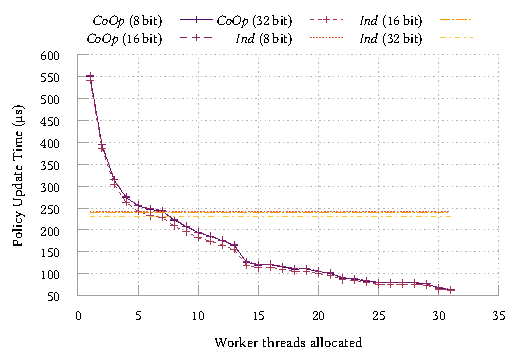
\includegraphics{plots/opal/rl-perf-tester/vary-core}
	}
	\caption{
		\Coopfw{}'s online learning performance improves with additional cores, on max size tasks (\num{129} work items). This requires \num{8} workers to offer greater online throughput than single-threaded in-NIC RL. Sharper performance increases occur when a new physical core is added (\numrange{7}{8}) or the scheduler works around a bottleneck (\numrange{13}{14}).\label{fig:vary-core}}
\end{figure}

\begin{figure}
	\resizebox{\resultplotwidth}{!}{
		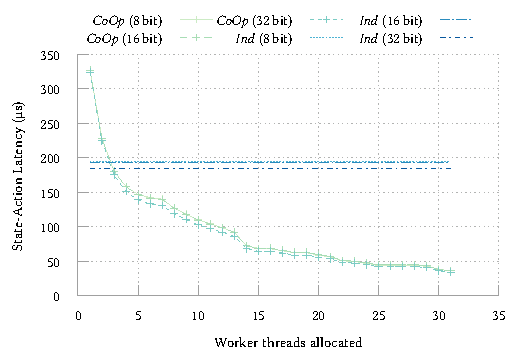
\includegraphics{plots/opal/rl-perf-tester/vary-core-latency}
	}
	\caption{\Coopfw{}'s action latencies similarly improve with more cores. This requires \num{3} workers (4 total contexts) to improve upon the state-action latency of single-threaded in-NIC RL.\label{fig:vary-core-latency}}
\end{figure}

\Cref{fig:vary-work,fig:vary-work-latency} show how policy complexity affects update cost and state-action latency respectively, scaling from a bias tile up to the full DDoS policy size.\footnote{Input vectors here all have 20 elements regardless of the policy design.}
\Coopfw{} always produces an action in less time than \Indfw{}, but requires at least one state-based tile to excel in online learning.
%We note that this is a trivial case, in that the use of \emph{only} a bias tile negates the need for any input state (similar to a multi-arm bandit problem).
We note that this is a trivial case, as using \emph{only} a bias tile returns a single preference list regardless of input state.

We found that a key aspect of in-NIC execution is that it allows far tighter bounds on tail latency compared to host offloading.
Examining the state-action latencies in \cref{tab:lats}, we see that \num{99.99}\nthscript{th} percentile latencies exceed the median by \qtylist{0.58;0.66}{\percent} for \Indfw{} and \Coopfw{}, respectively.
Similar results were observed for other bit depths.
By contrast, host-based tail latencies are at least \qty{40.53}{\percent} greater even when the parallel worker count is at or below the physical core count.
We show the cumulative distributions of these in detail (\cref{fig:lat-cumul}), noting how just one additional CPU-intensive task---potentially automated system updates, scans, or another vNF/traffic processing task---impacts tail latencies further (\emph{Float(Over)}).

\begin{figure}[t]
	\resizebox{\resultplotwidth}{!}{
		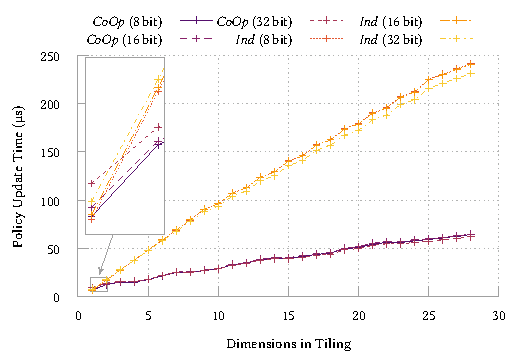
\includegraphics{plots/opal/rl-perf-tester/vary-work}
	}
	\caption{\Coopfw{} fully processes updates faster than \Indfw{}---thus has higher online performance---on almost all policy sizes. Lower bit depths are more effective on simpler policies.\label{fig:vary-work}}
\end{figure}

\begin{figure}
	\resizebox{\resultplotwidth}{!}{
		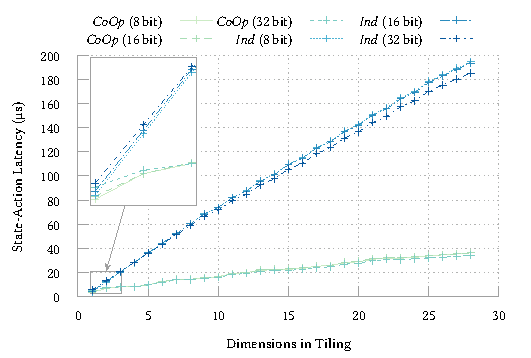
\includegraphics{plots/opal/rl-perf-tester/vary-work-latency}
	}
	\caption{State-action latency scales with additional work in a similar manner to overall processing time; though \qty{32}{\bit} firmwares become more effective sooner (at \num{3} work items).\label{fig:vary-work-latency}}
\end{figure}

\begin{figure}
	\centering
	\begin{subfigure}{\linewidth}
		\resizebox{1.0\linewidth}{!}{
			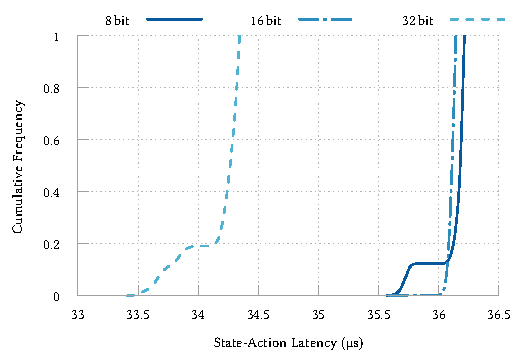
\includegraphics{plots/opal/rl-perf-tester/latency-cumul-thesis}
		}
		\caption{\approachshort's \Coopfw{} design achieves consistent, tight latency bounds.}
	\end{subfigure}

	\begin{subfigure}{\linewidth}
		\resizebox{1.0\linewidth}{!}{
			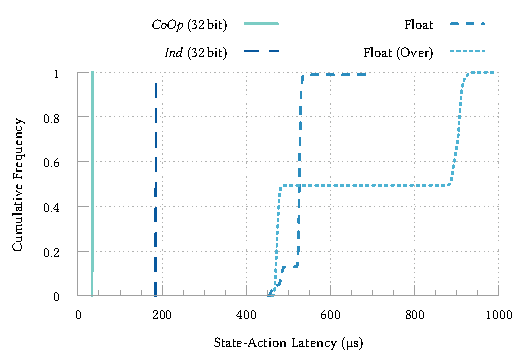
\includegraphics{plots/opal/rl-perf-tester/latency-cumul-broad-thesis}
		}
		\caption{Tail latencies suffer in hosts---particularly when oversubscribed.}
	\end{subfigure}
	\caption{Cumulative state-action latency plots for \approachshort{} and host-based execution.\label{fig:lat-cumul}}
\end{figure}

A noteworthy trend is that \qtylist{8;16}{\bit} versions of \approachshort{} consistently underperform compared to \qty{32}{\bit}, except for smaller workloads (seen in the zoomed portions of \cref{fig:vary-work,fig:vary-work-latency}).
This occurs even though our implementation is optimised to read and write policy data in batches (achieving fewer I/O operations).
We see this because the native register width on the NFP is \qty{32}{\bit}, and so the compiler must emit extra instructions around arithmetic operations to correctly load and update values.
This matches \qty{32}{\bit} becoming dominant in complex workloads: higher dimension tilings require more arithmetic operations.
Most of the I/O comes \emph{after} this step, causing ALU use to dominate.
This also explains why \qty{32}{\bit} becomes the best choice at different policy complexities for online (\cref{fig:vary-work}, 10 dims) and offline (\cref{fig:vary-work-latency}, 3 dims) agents, where hashtable accesses and a \texttt{memcpy} of the state vector fall into the serial portion of the online algorithm.
Smaller bit depths still give a \qtyrange{2}{4}{\times} saving in memory for policy storage (enabling more fine-grained or complex policies), in exchange for slightly worse latency and throughput.
To overcome this, we investigated bit-stuffing several values into a single word during atomic writeback (as the platform offers both \qtylist{32;64
}{\bit} atomic addition).
This is analogous to SIMD through clever use of padding bits, but we found that manipulating tiles into the correct format added \qty{10}{\percent} extra overhead.

\subsection{Work allocation}
\Cref{fig:work-alloc-32} shows that our heuristic allocator (\emph{Balanced}) is key in achieving consistent sub-\qtylist{35;65}{\micro\second} latencies/update times, respectively.
The trend is repeated for all bit depths.
The constant difference between \emph{Action} and \emph{Update Prep} scales linearly with bit depth, matching storage and lookup work in the serial portion of \emph{ParSa} (plots omitted).
The severe underperformance of the \emph{Na\"{i}ve} allocator confirms that work item complexity is correlated with its index, as batching work in contiguous chunks gives some workers only high-dimensionality tilings.
The minor gap in lower bound performance between the \emph{Random} and \emph{Balanced} allocators suggests that further optimisations can be made.
We expect that closing or exceeding this gap may require more complex modelling of hardware thread interactions, which lies far beyond the scope of in-NIC scheduling.
Some additional complexity may be tolerated, subject to code store limits---scheduling runs exactly once per configuration change, so does not impact per-action code.

\begin{figure}
	\resizebox{\resultplotwidth}{!}{
		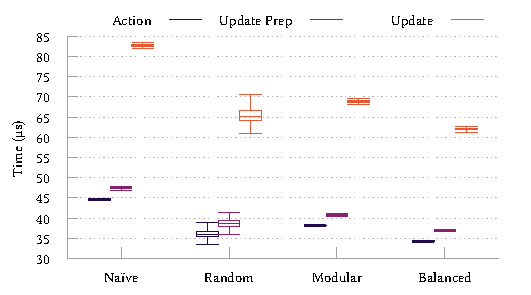
\includegraphics{plots/opal/rl-perf-tester/work-strat-32bit}
	}
	\caption{Action/update compute times in a \qty{32}{\bit} \Coopfw{} agent under different work schedulers.\label{fig:work-alloc-32}}
\end{figure}

\begin{figure}
	\resizebox{\resultplotwidth}{!}{
		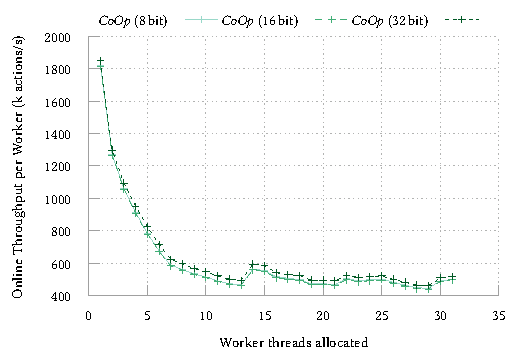
\includegraphics{plots/opal/rl-perf-tester/vary-core-tput-on-per}
	}
	\caption{Throughput per added worker in a \Coopfw{} agent.\label{fig:tput-per-core}}
\end{figure}

An interesting aspect of \Coopfw{} and \emph{ParSa} is that adding cores has both diminishing returns and key thresholds to pass.
Consider \cref{fig:tput-per-core}, where the throughput per worker decreases with cores but occasionally increases sharply.
Later downward ticks (\numrange{25}{29} workers) correspond to plateaus in throughput.
This is a problem stemming from the granularity of work items (i.e., tilings in \emph{ParSa}), where our scheduler cannot find a better solution to a bottleneck until extra cores are allocated.
We measured individual work items in state-action computation to take a mean \qtylist{5.2; 6.2; 9.7; 11.0}{\micro\second} for bias, CLS, CTM and IMEM tilings respectively.
Though we have a \qty{4.2}{\times} factor of task oversubscription, it is clear that latencies are eventually bound below by the length of the longest task.

\subsection{End-to-end RL latency}
%?? PCIe RTT is 10us (neugebauer, BNN NFP paper), NFP RTT is 18us (own measurements). EMEM Ring one-way is 120ns.
%?? Cziva~\parencite[pp.113]{DBLP:phd/ethos/Cziva18} discusses vNF times.
%?? reference the inference times brought up in Taurus?
Referring to \cref{fig:state-slip}, we take $t_2$ from \cref{tab:lats} for host and in-NIC processing times, and substitute $t_1+t_3$ for the state packet round-trip time to the decision site:
\begin{description}
	\item[In-NIC.] As described in \cref{sec:agent-environment-communication}, EMEM rings have a median one way delay cross-island of \qty{140}{\nano\second}, giving a \emph{median \qty{34.63}{\micro\second} end-to-end inference latency}.
	\item[Dedicated Collector.] Offloads hosted in this manner will employ DPDK to maximise performance, giving one-way PCIe delays of \qtyrange{0.9}{2.3}{\micro\second} for network packets~\parencite{DBLP:conf/sigcomm/NeugebauerAZAL018}.
	A UDP packet carrying \num{20} elements of state in \approachshort{} is \qty{128}{\byte}, so costs \qty{1}{\micro\second} to forward, and the reply state-action pair is slightly larger.
	\emph{This gives an end-to-end inference latency of \qty{517.9}{\micro\second}}.
	\item[vNF Offload.] \Textcite{DBLP:journals/cm/CzivaP17} show that more lightweight vNF frameworks like GNF~\parencite{DBLP:journals/cm/CzivaP17} and ClickOS~\parencite{DBLP:conf/nsdi/MartinsAROHBH14} add \qtyrange{45}{55}{\micro\second} \emph{additional} RTT latency above PCIe costs.
	\emph{This gives an end-to-end inference latency of \qty{572.9}{\micro\second}}.
\end{description}
Using these estimates, in-NIC classical RL inference offers \qtylist{14.96;16.54}{\times} speedups in latency over collector and vNF deployments respectively (assuming no steering cost in either case).
We also contrast these against deep RL policies on network tasks, which can take \qty{3}{\milli\second} to compute~\parencite{DBLP:journals/corr/abs-1910-04054}---2 orders of magnitude above \approachshort{} with identically sized (20-dim) input vectors.
%In the name of fairness, we assume that rule installation uses same mechanism we recommend, but show how bad it can get? I.e. with rule installation costs etc.

\subsection{Co-existence with the dataplane}
Our setup met \qty{40}{\giga\bit\per\second} for packet sizes $\ge$\qty{256}{\byte}.
%For frame sizes of \qtylist{64;128;256}{\byte} input traffic rates were \qtylist{17.4;32.9;37.0}{\giga\bit\per\second} respectively (\qtylist[per-symbol=p,sticky-per=true]{33.9;32.2;18.1}{\mega\packet\per\second}).
For frame sizes of \qtylist{64;128}{\byte}, input traffic rates were \qtylist{17.4;32.9}{\giga\bit\per\second} respectively (\qtylist[per-symbol=p,sticky-per=true]{33.9;32.2}{\mega\packet\per\second}).
Passing this traffic over the NFP device running \approachshort, no packet losses were incurred at any rate of RL actions.

We show the effect of RL workloads on the round-trip latencies of cross traffic through \cref{fig:dataplane-coop}.
As observed latencies do not obey a normal distribution (particularly \qtylist{256;1518}{\byte}, which are bimodal), we employ a one-tailed \emph{Mann-Whitney U test} to mark statistically significant population increases in latency ($p < 0.05$) with a ``+''.
In general, statistically significant latency increases concentrate around smaller packet sizes.
All (bar one) of these affected \nth{99} percentile latencies by under \qty{0.38}{\percent} (at most \qty{78}{\nano\second}).
This slight degradation can be explained by increased pressure on the NFP's \emph{Command Push-Pull} (CPP) bus, which is responsible for handling cross-island accesses to memory (particularly IMEM/EMEM) and other resources.
\approachshort{} places load on the CPP bus through its \inring{}/\outring{} EMEM rings and last-tier policy accesses.
This also explains the sensitivity of \qty{256}{\byte} packets to \approachshort{}---the NFP P4 toolchain segments packets, storing metadata (e.g., MAC prepend) and the first bytes of a packet in a \qty{256}{\byte} CTM block and parking their payloads in EMEM.
\qty{256}{\byte} packets overshoot this due to metadata, causing small I/O accesses at a high rate for packets sized around this cutoff.
%Regardless, this effect is small when observed.

The anomalous result is \qty{128}{\byte} packets at \num{3000} RL action/update computations per second, causing a \qty{222}{\nano\second} (\qty{1.18}{\percent}) increase, shown in \cref{fig:dataplane-example}.
This is observed through a shift of some packet latencies from the mode towards the tail, but no other changes in the distribution.
In the above context, we believe that the inbound request rate is weakly synchronised with inbound packets, causing a higher level of burstiness around accesses to the CPP bus.
We expect that dedicated hardware/FPGA designs can avoid this problem by having dedicated \inring{}/\outring{} access mechanisms for an \approachshort{} agent.

\begin{figure}
	\centering
	\begin{subfigure}{0.45\linewidth}
		\resizebox{1.0\linewidth}{!}{
%			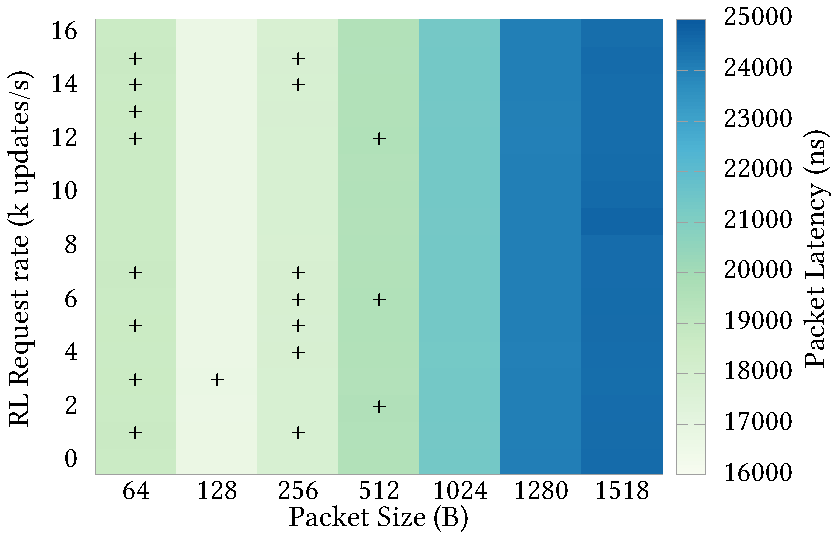
\includegraphics{../plots/build/stress/heat-latency-median}
			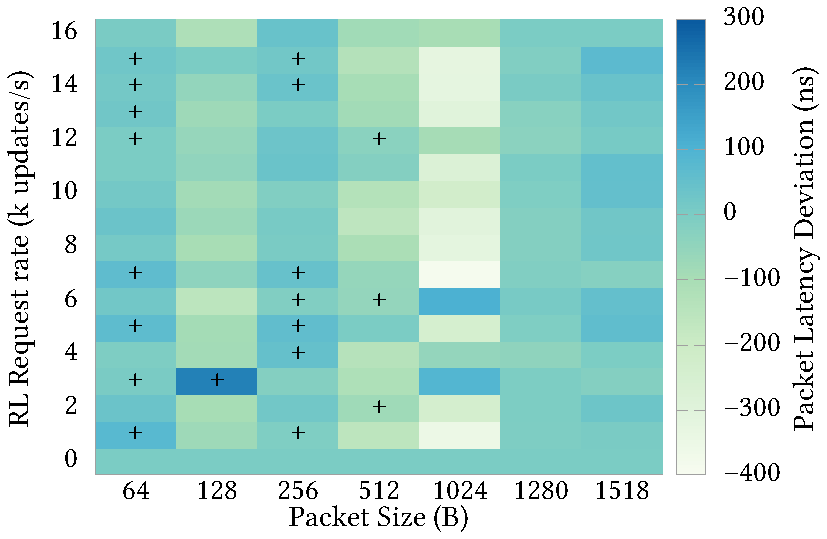
\includegraphics{plots/opal/stress/heat-latency-two-9-rel}
%			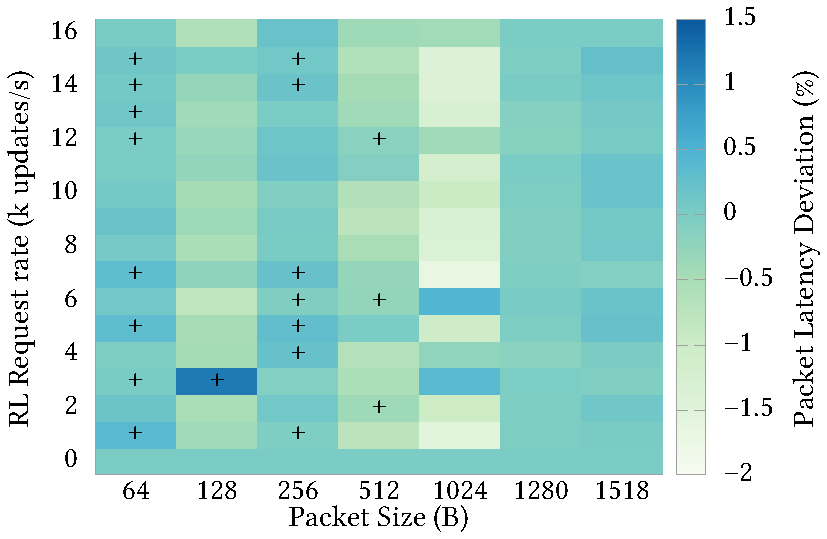
\includegraphics{../plots/build/stress/heat-latency-two-9-perc}
		}
		\caption{Deviations in \nth{99} percentile cross-traffic RTTs.\label{fig:dataplane-heat}}
	\end{subfigure}
	\hspace{0.05\linewidth}
		\begin{subfigure}{0.45\linewidth}
		\resizebox{1.0\linewidth}{!}{
			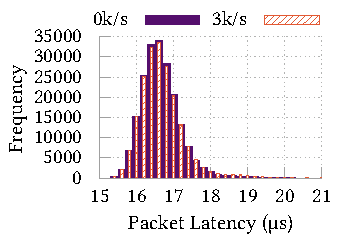
\includegraphics{plots/opal/stress/histo-128B-0-3-trim}
		}
		\caption{Distribution of RTTs for \qty{128}{\byte} packets for \numlist{0;3000} RL actions/s.\label{fig:dataplane-example}}
	\end{subfigure}
	\caption{Effects on tail latency of cross-traffic caused by different loads of off-path RL compute. Statistically significant increases in population latency are concentrated on smaller packet sizes, and are typically sub-\qty{78}{\nano\second}.\label{fig:dataplane-coop}}
\end{figure}

\subsection{Resource requirements}
\Cref{tab:resources} shows how \approachshort{} consumes shared memory as it scales to fit a device's compute resources, compared with a simple P4 forwarding application.
As one program is installed per ME, these results represent the minimum and maximum resource use on a single island (i.e., without replacing P4 workers).
We observe negligible costs on shared EMEM ($\sim$\qty{4}{\mebi\byte}), incurred due to hashtables for past state and rewards.
The most significant costs arise due to policy data (\qty{405}{\kibi\byte} shared IMEM, \qty{90}{\kibi\byte} local CTM, \qty{15}{\kibi\byte} local CLS), which can be halved or quartered using \qtylist{16;8}{\bit} quantisation and remain constant regardless of compute unit usage.
This is a high upfront cost on per-island resources (CLS/CTM)---\approachshort{} leaves resources for other off-path dataplane applications, but is fairest from 3 cores onwards.

%Thread local storage in CLS for compute/register spilling scales with the number of MEs required (requiring \qtylist{13.77;15.49}{\percent} per-ME for \Indfw{}/\Coopfw) due to precaching and the space needed to hold tile lists.
%Due to the initial policy cost this falls below the fair share at 3 MEs, but always allows for co-existence with other asynchronous dataplane programs.

\begin{table}
\caption{NFP memory use due to \approachshort{} using \numlist{1;4} MEs (\qty{32}{\bit}). CLS and CTM are shared between all programs on the same island (placing our RL agent on i5), while EMEM and IMEM are shared between all NFP programs on a NIC.\label{tab:resources}}
\resizebox{\linewidth}{!}{
\begin{tabular}{
		@{}c
		S[table-format=4.2] S[table-format=2.2]
		S[table-format=4.2] S[table-format=2.2]
		S[table-format=4.2] S[table-format=2.2]
		S[table-format=2.2] S[table-format=2.2]
		S[table-format=3.2] S[table-format=2.2]
		@{}
	}
	\toprule Firmware & \multicolumn{2}{c}{EMEM} & \multicolumn{2}{c}{EMEM Cache} & \multicolumn{2}{c}{IMEM} & \multicolumn{2}{c}{i5.CLS} & \multicolumn{2}{c}{i5.CTM}\\
	& \multicolumn{1}{c}{\si{\mebi\byte}} & \multicolumn{1}{c}{\si{\percent}} & \multicolumn{1}{c}{\si{\kibi\byte}} & \multicolumn{1}{c}{\si{\percent}} & \multicolumn{1}{c}{\si{\kibi\byte}} & \multicolumn{1}{c}{\si{\percent}} & \multicolumn{1}{c}{\si{\kibi\byte}} & \multicolumn{1}{c}{\si{\percent}} & \multicolumn{1}{c}{\si{\kibi\byte}} & \multicolumn{1}{c}{\si{\percent}} \\
	\midrule Base P4 & 6776.67 & 88.24 & 268.52 & 2.91 & 858.28 & 10.48 & 0.00 & 0.00 & 0.00 & 0.00 \\
	\Indfw(1) & 6780.21 & 88.28 & 2541.08 & 27.57 & 1263.28 & 15.42 & 24.75 & 38.67 & 94.25 & 36.82 \\
	\Indfw(4) & 6780.22 & 88.28 & 2545.33 & 27.62 & 1263.28 & 15.42 & 51.18 & 79.97 & 107.00 & 41.80 \\
	\Coopfw(1) & 6779.12 & 88.27 & 1773.59 & 19.24 & 1263.28 & 15.42 & 22.41 & 35.01 & 90.00 & 35.16 \\
	\Coopfw(4) & 6779.12 & 88.27 & 1769.84 & 19.20 & 1263.28 & 15.42 & 52.16 & 81.49 & 90.00 & 35.16 \\
	\bottomrule
\end{tabular}
}
\end{table}

%\paragraph{The impact of bit depth}
%?? \Cref{fig:quant-acc}
%?? \qty{5}{\bit} mantissa suffices for $\ge$ \qty{90}{\percent} relative accuracy, so \qty{8}{\bit} is fine (1S + 2E + 5M), \qty{16}{\bit} is better.
%
%\begin{figure}
%	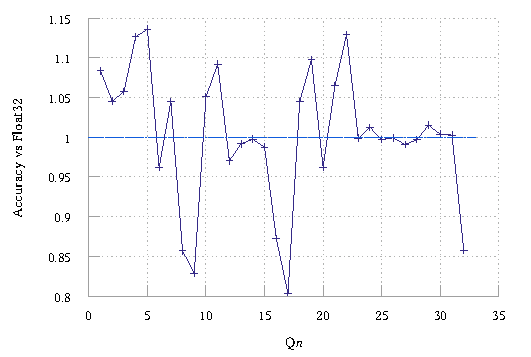
\includegraphics{../plots/build/marl-quant/accuracy-binary}
%	\caption{Normalised accuracy of a converted, pre-trained floating-point tile-coded policy after conversion to $32Qn$ fixed-point.}\label{fig:quant-acc}
%\end{figure}

\subsection{Deployability}
Setup of \approachshort{} uses two packet types: \emph{setup}, which contains learning (hyper-)parameters and most aspects of a policy, and \emph{tiling}, which provides a list of state indices for tiling sets.
We found that setup and tiling packets take a mean \qtylist{27.03;16.69}{\micro\second} to be processed on \Indfw{}, allowing an agent to be swapped between online and offline operation (or repurposed for another task) painlessly.
Online/offline swaps are useful when an agent should cease learning (i.e., when performance has converged), or if a change in the environment suggests that more training is needed.
Tiling packet processing scales linearly with the number of \emph{tiling sets}, due to the needed precaching of tile set boundaries.
Online-offline swaps for \Coopfw{} exhibit similar cost, however the need for explicit scheduling means that policy/tiling \emph{structure} changes (including the first complete setup) take \qty{422.63}{\micro\second} for the full-size policy described above.
The time taken for \Coopfw{} to schedule its tasks was found to scale with the number of workers ($m$) and work items ($n$) as described earlier (\cref{sec:work-allocation}, $\mathcal{O}{\left(n\log{m}\right)}$).
Ignoring the trivial solutions, reducing the worker count to \num{1} costs a mean \qty{238.22}{\micro\second}, while placing a single task incurs \qty{53.79}{\micro\second}.
Policy \emph{data} changes require no additional work in any case, resolving purely to \texttt{memcpy}s.

We observed that firmware installation (i.e., changing from \Indfw{} to \Coopfw{}, bit depth, or increasing maximum policy sizes) took a mean time of \qty{38.83}{\second}.
In the event that appropriate firmwares are not pre-compiled, we found that compiling and linking both \approachshort{} and the P4 toolchain took around \qty{35}{\second}, while changing only \approachshort{} parameters required around \qty{25}{\second}.
These results show that \approachshort{} can be easily adapted and altered by network administrators once in place, and illustrates an advantage of SoC-based SmartNICs.

\subsection{Magnitude comparisons against PDP ML}
?? Rework a bunch of "Related Work" into here.


\section{Potential Integrations}\label{sec:opal-potential-integrations}
To show the applicability and use of \approachshort{}, we propose an ideal integration which would benefit from in-NIC RL; online DDoS attack mitigation.
We support this using other state-of-the-art P4/PDP developments, and discuss how best to balance the concerns of online training (\Coopfw{} agents) with throughput (\Indfw{} agents) in widespread deployment.
%Additionally, we discuss how network administrators may combine offline (\Indfw) and online (\Coopfw) agents to achieve online learning while maximising action throughput in the majority of the network.

%?? How do we move this intuition to the start? ELI5 as dimitris says, to get the full end-to-end pipeline across to the reader.

\subsection{In-Network DDoS Defence}\label{sec:integ-1}
Classical RL has seen recent use in real-time, adaptive DDoS mitigation~\parencite{DBLP:journals/tnsm/SimpsonRP20}.
\Citeauthor{DBLP:journals/tnsm/SimpsonRP20}'s \emph{Guarded} agent design uses a mixture of global network state and local, per-flow state to monitor how flows respond to bandwidth changes and packet drop---applying the observations made by SPIFFY~\parencite{DBLP:conf/ndss/KangGS16} (observing how flow behaviour reacts to a change in rate limits) with more allowance for congestion-unaware protocols.
Actions then move flows up or down in punishment levels according to a finite state machine.

\fakepara{Why in-NIC?}
This approach relies on co-hosting traffic measurement and analysis alongside OpenFlow-compatible switches at the edge nodes of an AS.
However, packet mirroring and offloading RL computation to a host (potentially over layers of virtualisation) are all sources of additional, consistent state-action latency.
Both traffic statistics collection \emph{and} data-driven learning must be executed on such hosts/network functions.
Unless running these stages in a dedicated pipeline (adding further processing latency), resource contention between these processes will further impact tail latencies.
Naturally, this requires high-performance hardware to be stacked at network egress points, potentially beyond reasonable space, power, or ventilation constraints.
The solution to implement and improve upon this work using \approachshort{} is to place its RL agents on SmartNICs at AS edge nodes---a bump-in-the-wire deployment.

%?? Any way to move some of this sooner? I.e., this is ``why move DDoS prevention here'', Stefanos suggested backporting some of this to justify ``why \emph{RL} in-NIC''?

\fakepara{Inputs}
To collate the required inputs and state, we then examine the recent innovations of the community.
Low-latency, pure-P4 solutions to extract and record per-flow TCP state directly in the dataplane such as Dapper~\parencite{DBLP:conf/sosr/GhasemiBR17} and Sonata~\parencite{DBLP:conf/sigcomm/GuptaHCFRW18} are well-studied.
In fact, the statistics offered by Dapper are a super-set of the local input state values employed by \emph{Guarded} agents, offering an opportunity to further improve their efficacy. 
We propose placing such monitors in the P4 dataplane, existing on-chip alongside the \approachshort{} agent.
The required global state (load measures from network paths) must still come from elsewhere in the network; this is now the element at highest risk of becoming stale, but the least likely to vary significantly in response to individual actions.

The original work uses theoretical ``ground truth'' rewards, whose correct implementation and designs were left as an open challenge. 
We posit that INDDoS~\parencite{tnms-ddos-victim-ident}, which uses Count-min Sketches to estimate DDoS victim cardinality, could be an effective reward function source---i.e., using the number of detected victims as a loss value.

\fakepara{Integrating \approachshort}
Before each monitoring action, we require that the table hosting this hybrid solution polls \approachshort{}'s \emph{\outring{} Ring} for any generated actions.
As we note in \cref{sec:limitations}, these actions would be placed into a small hash table and simultaneously exported to the attached controller to be inserted as P4 rules in batches.
Afterwards, packet ingress timestamps would be used to emulate the \emph{Timed Random Sequential} (TRS) scheduler used by the anti-DDoS agents for rate-controlled work, where state vectors would be selected and passed into \approachshort.
By design, active flows which are not \emph{judged} after a configurable time are discarded to prune the work set and allow new flows to be seen by the agent.
The tight bounds on execution time known \emph{a priori} make it easy to calculate the maximum number of decisions which can be made per deadline.
Reward values would then be separately inserted by a modified INDDoS table.

%?? Can I have a P4 code snippet here?

Reducing state-action latency (i.e., with \Coopfw) is useful for minimising the noise inherent in learning.
However, an agent is limited by the fact that it can take at least one RTT for meaningful changes to occur in a flow's behaviour ($\mathcal{O}{\left(\si{\milli\second}\right)}$ in a transit AS/ISP).
Accordingly, this use-case benefits most from an increase in \emph{throughput} using \Indfw{}.
In this context, higher throughput means that network flows are more likely to be judged in every timestep, even when flow cardinality is high---making it more likely that changes in flow behaviour will be observed, acted on, and learned from.

We note that the TRS scheduler is designed to handle large numbers of attack flows, combining seen state vectors over time while the asynchronous agent is itself busy.
A number of (attack) flows beyond the maximum throughput simply makes it take longer in expectation for a flow to be reassessed.
As shown in \cref{sec:evaluation}, \approachshort{} far exceeds the throughput of host offloading.
The control plane can then use wildcards or specific matches to narrow down or expand the set of flows to be controlled dynamically, though explicit (TRS) scheduling is still key in such adversarial environments.

%\subsection{Something host-specific?}\label{sec:integ-2}
%Accelerate something at an end-host... Flow control? Something datacentre-y? A novel CCA? What?

\subsection{Network Deployment Considerations}
The two compute models discussed above need not be homogeneously deployed.
In a networked deployment, a subset of \approachshort{} nodes could be \coopfw{} agents, training online, while most other nodes run \indfw{} designs to meet throughput guarantees.
The control plane would then combine, downsample, and distribute these improved policies between offline agents.
This can be taken further still, using policy deltas or execution traces to enable out-of-path transfer learning for more complex models such as neural networks.

%\section{Related Work}
%%?? Try and compare my work here when possible?

\fakepara{DDoS Prevention}
\Textcite{DBLP:conf/lcn/BragaMP10} examine the detection of flooding DDoS attacks through \emph{self-organising maps}, using SDN to gather statistics effectively.
Many of their features aren't overly relevant, as their focus is not active defence or discovering \emph{which} hosts contribute to an attack.
%?? Actually talk about Marl (???) to appease reviewer \#1.
The closest available approach within this field is that of \textcite{DBLP:journals/eaai/MalialisK15} (whom we have positioned our work against), and their contribution in applying RL to the task of intrusion prevention is significant: their work helps to show the viability of live, adaptive, feedback-loop-like control of the network to detect and prevent DDoS attacks.
They create a tree overlay topology (subdivided into teams), where each agent applies packet drop to \emph{all} flows inbound to a protected server.
%?? Recap their flaws, since they've been cut form every other aspect.
Our results show that their technique underperforms at high host density and when congestion-aware traffic dominates---that their results do not demonstrate this suggests an evaluation driven purely by traces (rather than live application dynamics).

\emph{SPIFFY} \cite{DBLP:conf/ndss/KangGS16} aims to remedy transit-link attacks by observing how flows from each source respond to a sudden increase in available bandwidth.
\Citeauthor{DBLP:conf/ndss/KangGS16} realise that bots participating in an attack are often unable to match this bandwidth expansion (having already saturated the capacity of their outbound links), while legitimate flows typically speed up to match the new fair-share rate.
%Attackers must either be detected or reduce the throughput of each bot, increasing the cost of launching an attack.
%Unlike our approach (and due to the class of attacks it is designed to defend against), SPIFFY is intended to be deployed within ASes, although .
A weakness of their approach is that computing a route to measure bandwidth expansion on real networks can be costly (up to \SI{14}{\second} for the Cogent topology), and that the low expansion factors in real network can require more ``rounds'' of filtering.
By contrast, our approach takes a constant time to compute an action for a flow regardless of topology size.
Their assumptions about traffic response to such bandwidth expansion do not hold for constant bitrate flows (e.g., VoIP) and may not extend to HTTP DASH flows, both of which make up a sizeable proportion of network traffic.

\emph{Athena} \cite{DBLP:conf/dsn/LeeKSPY17} is a generalised SDN framework for intrusion detection, but has shown the use of a \emph{k-nearest neighbours} classifier to detect individual attack flows.
Although heavyweight (and proven to be effective compared with \textcite{DBLP:conf/lcn/BragaMP10}), their comparison against SPIFFY lacks the quantitative evidence required to understand how the system compares.
\Textcite{DBLP:conf/sp/SmithS18} use AS-level routing to tackle both transit-link and flooding-based attacks.
This view is taken due to the perceived cost of per-stream classification and inherent sensitivity to adversarial examples.
The approach is creative, relying upon BGP \emph{fraudulent route reverse poisoning} to preserve traffic to a target AS, but unlike SPIFFY the approach doesn't actually \emph{remove} the congestion.
Because of this, flooding-based attacks aren't fully alleviated.

%?? Abuses of RL 
\fakepara{RL in Networks}
Earnest, well-considered application of RL towards the challenge of intrusion prevention has seen comparatively little examination.
Past work treats the paradigm as a traditional classifier for anomaly detection \cite{shamshirband2014anomaly} and DDoS prevention \cite{DBLP:conf/mates/ServinK08}.
Given that the main strengths of RL techniques are the ability to control ongoing interaction and adapt by observing the concrete effects of actions, such works don't apply the rich literature on the subject to its fullest potential.

For categorising how RL fits into solving problems, we label works as direct- or indirect-control RL.
A \emph{direct-control} RL problem is one where the RL agent(s) learn optimal control over a set of actions as the \emph{primary} defence or decision-maker---requiring measurements, reward functions and action sets tailored for this purpose.
%We feel there is a shortage of work in this category at present, at least in the field of networks.
To date, the best-fitting example we have encountered is that of \textcite{DBLP:journals/eaai/MalialisK15}.
An \emph{indirect-control} RL problem is one where agents act in service to \emph{another technique} responsible for decision-making, optimising or generalising aspects of its operation beyond that of hand-coded heuristics.
A past example includes learning when best to share knowledge between \emph{hidden Markov model} anomaly detectors \cite{DBLP:conf/paisi/XuSH07}.
%The position of this work is weakened by its reliance on the problematic `DARPA99' dataset \cite{DARPA-IDD, DBLP:conf/cisda/TavallaeeBLG09, DBLP:conf/sp/SommerP10}, but the idea itself is well-treated and this acts as a driver for improvements in this direction.
This work is weakened by its reliance on the problematic `DARPA99' dataset \cite{DBLP:conf/sp/SommerP10}, but the idea itself is well-treated.
Outside of intrusion detection, there has been growing interest in the use of RL in data-driven networking, such as for intra-AS route optimisation \cite{DBLP:conf/hotnets/ValadarskySST17} and resource-constrained process allocation \cite{DBLP:conf/hotnets/MaoAMK16}.
\textcite{DBLP:conf/sigcomm/MaoNA17} employ client-side observations of network state and video performance with RL to optimise bitrate selection for multimedia streaming.
\emph{AuTO} \cite{DBLP:conf/sigcomm/ChenL0L18} employs deep RL to perform traffic optimisation.
Crucially, they find that the vast majority of flows are short-lived, requiring effective decisions in less than a millisecond.
To overcome the high latency of action computation via a neural network, two agents are trained, handling aspects of short and long flows respectively.
The first learns to optimise the flow size thresholds to demarcate long and short flows; these short flows are routed by ECMP.
The second agent makes bespoke decisions about routing, prioritisation etc.\ for each of the remaining long flows.


\section{Summary}\label{sec:opal-summary}
%?? Please rewrite me to be thesis-y, not sales-y.

%We have presented \emph{\approachshort{}}, bringing \emph{online reinforcement learning} to the dataplane.
%\approachshort{} has shown how classical RL techniques make online learning possible by simplifying update logic and enabling parallel processing.
%In-\gls{acr:nic} use of these algorithms enabled a \qtyrange{15}{21}{\times} reduction in median--\num{99.99}\nthscript{th} inference times and order of magnitude improvement in online learning throughput compared to host offloading.
%The deployment environment and asynchronous design were shown to eliminate \gls{acr:pcie} delays and impose minimal impact on carried dataplane traffic.
%We also showed how \approachshort{} scales with additional compute resources at deployment to improve on decision latency and throughput.
%Our throughput-optimal design, \Indfw{}, improves upon these metrics with \emph{just one worker}.
%
%In future, we aim to examine the performance of individual applications driven by \approachshort---both classical and \gls{acr:drl}-based---and how a NetFPGA implementation can offer further latency and throughput improvements.
%A promising avenue here would be to investigate constant transfer learning between online \approachshort{} agents and high-throughput offline function approximators such as \glspl{acr:bnn}.

%?? We stress that none of the other approaches listed here (or that we have seen) tackle the issue of \emph{online learning and control} in-network---we believe \approachshort{} has broken new ground in this regard.
%
%??
%
%?? Key: Scale back algos and data to enable...

We have seen through this chapter that online \gls{acr:rl} in \gls{acr:pdp} hardware is not only possible, but crucially offers tangible improvements to state-action latency and online learning throughput.
This confirms one of the key assertions in my thesis statement, namely that \superrecallthesis{2}.
The key to doing so was to consider the architectural strengths and weaknesses of the target environment---in this case, SmartNIC devices---to creatively choose data formats and algorithms which suit their weaker, \gls{acr:fpu}-free, resource constrained environment rather than the state of the art.
We have considered an off-path execution model, which places \gls{acr:rl} logic in-\gls{acr:nic}, and have explored its essential role in preventing any impact to packet forwarding performance while enabling access to device-local state.
By looking at these both, in tandem with the high degree of parallelism that SmartNIC devices engender, the \emph{ParSa} algorithm was developed, which exploits the nature of tile-coded function approximation.
Moreover, I've shown that it subdivides into neatly disaggregated tasks and is thus wait-free when combined with an atomic aggregation mechanism.
We have examined two concrete implementations of \approachshort{}---\indfw{} and \coopfw---which apply SmartNICs' parallelism in different ways to tailor state-action latency or online and offline throughput according to operators' needs.
These are driven by effective methods for storing policy data across a non-uniform memory architecture, efficient internal and external communication, and careful task scheduling.
\approachshort{} was empirically evaluated on a number of benchmarks sized to large policies, confirming its reduced state-action latency and increased throughput compared to host-based execution.
Observed performance numbers justified design choices in the scheduler, and validated the off-path execution model's ability to protect other cross-traffic carried by the NIC.
Moreover, \approachshort{}'s runtime costs exist on a similar order of magnitude to existing \gls{acr:pdp} \gls{acr:ml} works implemented on the same hardware, indirectly confirming its validity and suggesting that sub \unit{\nano\second} execution might be offered by bespoke \gls{acr:fpga} implementations.
Finally, we have discussed how \approachshort{} might combine with other state-of-the-art \gls{acr:pdp} works to realise the anti-\gls{acr:ddos} agents presented in \cref{chap:ddos-rl} entirely in \gls{acr:pdp} hardware.

